% SPECIAL THANKS TO MICHAL MARTYNIAK (micmarty)
\documentclass[10pt,twoside,a4paper,hidelinks]{article}
\usepackage[utf8]{inputenc}

\usepackage{fontspec}                 % żeby ustawić czcionkę na systemową (Arial)
\usepackage{geometry}                 % do marginesów
\usepackage{indentfirst}              % żeby pierwsze akapity też miały wcięcie
\usepackage{titlesec}                 % żeby formatować tytuły rozdziałów itd.
\usepackage{secdot}                   % aby dodać kropkę za numerkiem podrzodziałów i podpodrozdziałów
\usepackage{chngcntr}                 % umożliwia numerowanie obrazków itp. względem rozdziału
\usepackage{tocloft}                  % umożliwia ustawienia dotyczące spisu treści i innych spisów
\usepackage{tabu}                     % do tabel
\usepackage[table,dvipsnames]{xcolor} % do kolorowania tabel
\usepackage{tabularx}                 % do lepszych tabel
\usepackage[backend=bibtex,language=polish,sorting=none,maxbibnames=99]{biblatex} % do bibliografii
\usepackage{enumitem}                 % do modyfikacji listy (begin{itemize}, niepotrzebne odstępy przed i po)
\usepackage{floatrow}                 % aby umożliwić wymuszenie położenia figury
\usepackage{caption}                  % do zmiany podpisów tabel i obrazków
\usepackage{setspace}                 % również do zmiany podpisów (konkretniej interlinii w podpisach - wymagany przez caption)
\usepackage{longtable}
\usepackage{booktabs}
\usepackage{tabu}
\usepackage{changepage}
\usepackage{amsthm}
\usepackage{hyperref}
\usepackage[final]{pdfpages}
\usepackage{multirow}
\usepackage[titletoc,title]{appendix}
\usepackage{listings}
% \usepackage{listingsutf8}
\usepackage{dirtree}
\usepackage{multicol}
\usepackage{subcaption}
\usepackage{amsmath,amssymb}
\usepackage{diagbox}
\usepackage{bm}
\usepackage{xcolor}
\usepackage{siunitx} % kąty w stopniach \ang{}
\usepackage{textcomp} % brackety dla dziedziny < > \textlange \textrangle
% Magia, żeby niezaleznie od wersji titlesec pokazywaly sie numery sekci i wszystkich innych
\usepackage{etoolbox}
\usepackage{polski}
\makeatletter
\patchcmd{\ttlh@hang}{\parindent\z@}{\parindent\z@\leavevmode}{}{}
\patchcmd{\ttlh@hang}{\noindent}{}{}{}
\makeatother
% koniec magii

\graphicspath{ {images/} }
\DeclareMathOperator{\EX}{\mathbb{E}} % expected value

% pokazanie jak można łamać słowa (hypenation)
\hyphenation{nisko-poziomowe}
\hyphenation{znaj-du-ją-cych}
\hyphenation{naj-bar-dziej}
\hyphenation{pa-ra-me-trów}
\hyphenation{sze-reg}
\hyphenation{naj-le-psze}
\hyphenation{Wrób-le-wskie-go}
\hyphenation{Sło-wiń-skie-go}
\hyphenation{Naj-częst-szyj-szymi}
\hyphenation{prze-te-sto-wa-no}
\hyphenation{Naj-wa-żniej-szym}
\hyphenation{naj-czę-stsze}
\hyphenation{wy-pro-wa-dza-nie}
\hyphenation{o-gra-ni-cze-niem}


% skroty
\newcommand{\abbrlabel}[1]{\makebox[3cm][l]{\textbf{#1}\ }}
\newenvironment{abbreviations}{\begin{list}{}{\renewcommand{\makelabel}{\abbrlabel}}}{\end{list}}

\newcommand\myicon[1]{{\color{#1}\rule{2ex}{2ex}}}
\newcommand{\myfolder}[2]{\myicon{#1}\ {#2}}
\newcommand\editnote[1]{\textcolor{red}{{\em [#1]}}} % See: https://tex.stackexchange.com/questions/9796/how-to-add-todo-notes


\definecolor{applegreen}{rgb}{0.55, 0.71, 0.0}
\definecolor{airblue}{rgb}{0.36, 0.54, 0.66}

\definecolor{listinggray}{gray}{0.9}
\definecolor{lbcolor}{rgb}{0.9,0.9,0.9}
        
\lstset{
  texcl=true,
  % To rozwiązanie z neta nie działa, a texcl działa
  % inputencoding=utf8x, 
  % extendedchars=\true,
  % literate={ą}{{\k{a}}}1
  %           {Ą}{{\k{A}}}1
  %           {ę}{{\k{e}}}1
  %           {Ę}{{\k{E}}}1
  %           {ó}{{\'o}}1
  %           {Ó}{{\'O}}1
  %           {ś}{{\'s}}1
  %           {Ś}{{\'S}}1
  %           {ł}{{\l{}}}1
  %           {Ł}{{\L{}}}1
  %           {ż}{{\.z}}1
  %           {Ż}{{\.Z}}1
  %           {ź}{{\'z}}1
  %           {Ź}{{\'Z}}1
  %           {ć}{{\'c}}1
  %           {Ć}{{\'C}}1
  %           {ń}{{\'n}}1
  %           {Ń}{{\'N}}1,
  backgroundcolor=\color{lbcolor},
  tabsize=4,
  language=C++,
  captionpos=b,
  tabsize=4,
  frame=lines,
  numbers=left,
  numberstyle=\tiny,
  numbersep=5pt,
  breaklines=true,
  showstringspaces=false,
  basicstyle=\linespread{0.94}\footnotesize\ttfamily,
% identifierstyle=\color{magenta},
  keywordstyle=\color[rgb]{0,0,1},
  commentstyle=\color{OliveGreen},
  stringstyle=\color{red}
  }


% Magia żeby dodatki miały ma początku "Dodatek X: ..."
\makeatletter
\renewcommand{\@redotocentry@pp}[1]{%
  \let\oldacl@pp=\addcontentsline
  \def\addcontentsline##1##2##3{%
    \def\@pptempa{##1}\def\@pptempb{toc}%
    \ifx\@pptempa\@pptempb
      \def\@pptempa{##2}\def\@pptempb{#1}%
      \ifx\@pptempa\@pptempb
        \oldacl@pp{##1}{##2}{\appendixname\space ##3}%
      \else
        \oldacl@pp{##1}{##2}{\chaptertitlename\space ##3}% added \chaptertitlename
      \fi
    \else
      \oldacl@pp{##1}{##2}{##3}%
    \fi}
}
\makeatother

% to jest jakas magia, aby odczytac szerokość longtable i ustawić tę wartość później jako LTcapwidth (parametr kontrolujący szerokość captiona w longtable)
% Creditsy i flaszkę proszę wysyłać do magika Heiko (http://compgroups.net/comp.text.tex/longtable-tablewidth/1922986)
\makeatletter
\newlength\LongtableWidth
\newcommand*{\org@longtable}{}
\let\org@longtable\longtable
\def\longtable{%
  \begingroup
    \advance\c@LT@tables\@ne
    \edef\x{LT@\romannumeral\c@LT@tables}%
    \global\LongtableWidth\z@
    \@ifundefined{\x}{%
      % longtable width not available
    }{%
      \def\LT@entry##1##2{%
        \global\advance\LongtableWidth##2\relax
      }%
      \@nameuse{\x}%
    }%
    % debug output
    \typeout{* \x: \the\LongtableWidth}%
  \endgroup
  \ifdim\LongtableWidth>\z@
    \setlength{\LTcapwidth}{\LongtableWidth}%
  \fi
  \org@longtable
}
\makeatother

% Rozpocznij od nowa numerowanie rysunków dla każdego rozdziału (section).
% Dodaje numer rozdziału do numeru rysunku: nr_rozdzial.nr_rysunku_w_ramach_rozdzialu
%
% Źródło: http://tex.stackexchange.com/questions/28333/continuous-v-per-chapter-section-numbering-of-figures-tables-and-other-docume
\counterwithin{figure}{section}

% to samo dla tabel
\counterwithin{table}{section}

% żeby nie było Rysunek tylko Rys
% \renewcommand{\figurename}{Rys.}

% żeby nie było odstępów przed/po/w środku listy (itemize, ew. dodać też dla enumerate?)
\SetLabelAlign{parright}{\parbox[t]{\labelwidth}{\raggedleft#1}}
\setlist[itemize]{noitemsep,nolistsep,topsep=0pt}
\setlist[description]{noitemsep,nolistsep,topsep=0pt,style=multiline,align=parright}

% ustawiamy domyślny odstęp przed i po pływającymi elementami (tabele i obrazki) umieszczonymi w środku tekstu (flaga H) na 0
\setlength{\intextsep}{0mm}
\setlength{\textfloatsep}{0mm}

% ustawiamy domyślną czcionkę dla podpisów na small (9pt dla article 10pt) oraz interlinię na 1.0
\captionsetup{font={small,stretch=1.0}}

% własny separator do podpisów (to, co jest po 'Rys. X.Y' - kropka, nazwana wewnętrznie jako 'dot')
\DeclareCaptionLabelSeparator{dot}{. }
\DeclareFloatVCode{6ptskip}{\vspace{6pt}}
\DeclareFloatVCode{12ptskip}{\vspace{12pt}}

% dla tabel: 0pt pod opisem, 6pt nad
\captionsetup[table]{singlelinecheck=false} % nie wyśrodkowywuj opisu w pojedynczej linii
\captionsetup[table]{labelfont=bf,labelsep=dot} % pogrubienie nagłówka podpisu (Tabela X.Y) i zakonczenie jej wczesniej zdefiniowana kropką
\floatsetup[table]{font={small,stretch=1.0},capposition=top,captionskip=0pt,precode=12ptskip,postcode=12ptskip} % nie wiem dlaczego, aby otrzymac odstep 6pt przed tabela, trzeba tutaj dac 12pt :/

\setlength{\LTpre}{12pt}
\setlength{\LTpost}{12pt}

\tabulinesep=2.0mm % wzięte z czapy, ale wygląda dobrze (minimalny odstęp między początkkiem i końcem wierwsza a jego zawartością - przydaje się w przypadku zawijanych wierszy)

% dla obrazków: 6pt nad opisem, 12pt pod
\captionsetup[figure]{justification=centering} % inaczej niz w tabelach - zawsze centruj podpis
\captionsetup[figure]{labelsep=dot} % użyj kropki jako separatora ale nie pogrubiaj
\floatsetup[figure]{capposition=bottom,captionskip=6pt,precode=12ptskip,postcode=12ptskip}

% koment do poniższych: bfseries oznacza pogrubienie, itshape kursywę, mdseries normalną
% large = 12pt, small = 9pt (zależne od ustawionego u góry podstawowego 10pt),
% normalsize podstawowy rozmiar czyli 10pt

% formatowanie tytułów rozdziałów (tutaj nazwane sekcjami)

\makeatletter
\newcommand{\setappendix}{Dodatek~\thesection:}
\newcommand{\setchapter}{\thesection.}
\titleformat{\section}{\bfseries\large}{%
  \ifnum\pdfstrcmp{\@currenvir}{appendices}=0
    \setappendix
  \else
    \setchapter
  \fi}{0.5em}{\MakeUppercase}
\makeatother


% formatowanie tytułów podrozdziałów (tutaj nazwane podsekcjami)
\titleformat*{\subsection}{\normalsize\bfseries\itshape}
\sectiondot{subsection}

% formatowanie tytułów punktów podrozdziałów (tutaj nazwane podpodsekcjami)
\titleformat*{\subsubsection}{\normalsize\itshape}
\sectiondot{subsubsection}

\titlespacing*{\section}{0pt}{12pt}{6pt}
\titlespacing*{\subsection}{0pt}{12pt}{6pt}
\titlespacing*{\subsubsection}{0pt}{12pt}{6pt}

% SPIS TREŚCI
% po polsku
\renewcommand{\contentsname}{Spis treści}

% żeby w spisie treści były też kropki po numerkach rozdziałów i podrozdziałów itd.
\renewcommand{\cftsecaftersnum}{.}
\renewcommand{\cftsubsecaftersnum}{.}
\renewcommand{\cftsubsubsecaftersnum}{.}
% żeby napis SPIS TREŚCI był wielkimi literami, pogrubiony itd
\renewcommand{\cfttoctitlefont}{\normalfont\large\bfseries\MakeUppercase}
% żeby tytuły rozdziałów w spisie oraz numery stron nie były pogrubione
\renewcommand\cftsecfont{\normalfont}
\renewcommand\cftsecpagefont{\normalfont}
% żeby dla rozdziałów też były kropki od napisu do numeru strony
\renewcommand\cftsecleader{\cftdotfill{\cftdotsep}}
% odstępy między akapitami 6pt
\setlength\cftbeforesecskip{6pt}
\setlength\cftbeforesubsecskip{6pt}
\setlength\cftbeforesubsubsecskip{6pt}
% żeby kropki od napisu do numeru strony były gęstsze
\renewcommand{\cftdotsep}{0}

% SPISY
% zmiana nazwy, czcionki, marginesu i separatora dla listy figur
\renewcommand{\listfigurename}{List of figures}
\renewcommand{\cftloftitlefont}{\normalfont\large\bfseries\MakeUppercase}
\setlength\cftbeforefigskip{6pt}
\renewcommand{\cftfigaftersnum}{.}

\setlength\cftfignumwidth{1.1cm}

% zmiana nazwa, czcionki, marginesu i separatora dla listy tabel
\renewcommand{\listtablename}{List of tables}
\renewcommand{\cftlottitlefont}{\normalfont\large\bfseries\MakeUppercase}
\setlength\cftbeforetabskip{6pt}
\renewcommand{\cfttabaftersnum}{.}

\setlength\cfttabnumwidth{1.1cm}

% zmiana nazwy z 'Bibliografia' na 'Wykaz literatury'
% \DefineBibliographyStrings{polish}{references = {Wykaz literatury}}
%\DeclareFieldFormat{labelnumberwidth}{#1\adddot\midsentence}
\DefineBibliographyStrings{polish}{references = {Wykaz literatury}}
\DeclareFieldFormat{labelnumberwidth}{#1\adddot\midsentence}
\DefineBibliographyStrings{polish}{urlseen = {data dostępu}}

% polskie rysunki
\renewcommand{\figurename}{Rys.}

% ustawienie marginesów
\geometry{
 a4paper,
 inner=3.5cm,
 outer=2.5cm,
 top=2.5cm,
 bottom=2.5cm
 }

\setmainfont{Arial}
\setlength{\parindent}{1.25cm}          % wcięcie przed akapitem
\renewcommand{\baselinestretch}{1.5}    % interlinia
\setlength{\parskip}{0pt}               % odległość pomiędzy akapitami

% żeby nie było wdów i sierot (linii samotnych ale nie słów!)
\widowpenalty10000
\clubpenalty10000

% komenda ignorująca cos w srodku tekstu (do naszych komentarzy)
\newcommand{\ignore}[2]{\hspace{0in}#2}

\theoremstyle{definition}
\newtheorem{definition}{Definition}[section]

\theoremstyle{remark}
\newtheorem*{remark}{Comment}

\bibliography{structure/bibliography}

\makeindex

\setcounter{page}{3} % rozpoczecie od strony 3

\begin{document}   % właściwy początek dokumentu
%\includepdf{STRONA_TYTULOWA_Z_MOJAPG.pdf}
\setcounter{page}{3}

\section*{Streszczenie}

Streszczenie \newpage
\section*{Abstract}

Abstract \newpage
\tableofcontents \newpage
\addcontentsline{toc}{section}{Wykaz ważniejszych oznaczeń i skrótów}
\section*{Wykaz ważniejszych oznaczeń i~skrótów}
\begin{abbreviations}
\item[RPI] Raspberry Pi
\item[USB] Universal Serial Bus
\item[HID] Human Interface Device
\item[CVE] Common Vulnerabilities and Exposures
\item[HTTP] Hypertext Transfer Protocol    
\item[UDP] User Datagram Protocol 
\item[TCP] Transmission Control Protocol 
\item[DNS] Domain Name Server
\item[DHCP] Dynamic Host Configuration Protocol
\item[MITM] Man in the middle
\item[CLI] Command Line Interface    
\end{abbreviations} \newpage

% %tutaj rozdzialy
 \section[Wstęp (Michał Krakowiak, Kacper Połom, Jakub Wyka)]{Wstęp}
Wraz z postępującą informatyzacją rośnie ilość zagrożeń na które narażone są współczesne systemy komputerowe.
Sprawia to, że coraz większą wagę przypisuje się odpowiedniemu zabezpieczeniu różnego rodzaju systemów komputerowych.
Wiele publikacji dotyczących tej tematyki traktuje o bezpieczeństwie aplikacji internetowych.
Jednak równie ważne jest testowanie podatności na fizyczne zagrożenia.
W związku z łatwiejszym dostępem do miniaturowej elektroniki w mediach można znaleźć informacje o złośliwych urządzeniach USB np. zaszytych w kablach~\cite{niebezpiecznik}.

\subsection[Cel pracy]{Cel pracy}
Z punktu widzenia osoby przeprowadzającej audyt bezpieczeństwa np. dla dużej korporacji, sprawdzenie bezpieczeństwa każdego pojedyńczego komputera w organizacji może być problematyczne.
Głównym celem projektu była realizacja dedykowanego systemu wspomagającego testowanie bezpieczeństwa systemów komputerowych.
Zaprojektowany system korzysta z odpowiednio oprogramowanych akcesoriów, które można przyłączyć do testowanego systemu po przez interfejs USB.
Są one w wstanie symulować działanie klawiatury i karty sieciowej. Możliwe scenariusze testowe, które mogą zostać zrealizowane to:
\begin{itemize}
    \item zatruwanie ustawień sieciowych
    \item przechwytywanie i/lub modyfikowanie ruchu sieciowego
    \item wprowadzanie zaprogramowanej sekwencji klawiszy
\end{itemize}
W celu zapewnienia użyteczności systemu przyjęliśmy założenie, że powinien on umożliwiać pracę zdalną np. z poziomu przeglądarki internetowej.

\subsection[Zawartość pracy]{Zawartość pracy}
W rozdziale~\ref{chapter:security} zostaną poruszone najważniejsze aspekty dotyczące testowania bezpieczeństwa.
Są to m.in.: podstawowe pojęcia wymagane do zrozumienia kontekstu pracy oraz kwestie regulacji prawnych, które  mają przedstawić różnicę między działaniami dozwolonymi a przestępstwem.
Ponadto omawiana jest problematyka bezpieczeństwem fizycznych interfejsów komputera.

W rozdziale~\ref{chapter:project} zawarty jest projekt realizowanego
systemu. Celem jego analitycznej części jest poznanie dziedziny problemu i 
wyróżnienie wymagań względem produktu. Następnie przedstawiany jest faktyczny projektu 
systemu zawierający diagram przypadków użycia, diagram klas oraz projekt interfejsu 
użytkownika.

Rozdział~\ref{chapter:enviroment}

Rozdział~\ref{chapter:usbkeyboard} skupia się na omówieniu realizacji funkcjonalności symulowania działania klawiatury USB.
Przedstawiony zostanie scenariusz użycia systemu.
Osobne podrozdziały poświęcono na opisanie mechanizmu, które pozwalają na kreowanie nowych urządzeń USB, oraz konfiguracji takiego urządzenia z wykorzystaniem systemu \textit{Linux} i języka programowania \textit{Python}.
Na koniec analizowane są aspekty, związane z wykryciem przez użytkownika działania realizowanego systemu lub potencjalnego zagrożenia.

Celem rozdziału~\ref{chapter:usbethernet} jest omówienie realizacji funkcjonalności 
symulowania działania karty sieciowej. Przedstawiona jest tam ogólna koncepcja 
funkcjonowania urządzenia w danej konfiguracji oraz szczegóły techniczne jej realizacji. 
W dalszej części opisana jest możliwość wykrycia złośliwego urządzenia w powyższej 
konfiguracj oraz dokładny opis realizowanych na nim scenariuszy testowych. 


Rozdział~\ref{chapter:results}


Z uwagi na stosunkowo niewielką liczbę dostępnych materiałów w języku polskim wykorzystano głównie anglojęzyczne źródła.
Spowodowało to problemy z tłumaczeniem terminologii.
Niektóre terminy nie posiadają polskiego tłumaczenia, w tym przypadku korzystano z oryginalnej nazwy.
Tam gdzie tłumaczenie istnieje, ale mogłoby wprowadzić niejednoznaczność przytacza się dodatkowo angielski odpowiednik. \newpage
\section[Testowanie bezpieczeństwa (Michał Krakowiak)]{Testowanie bezpieczeństwa}

Tematyka realizowanego projektu jest ściśle związana z bezpieczeństwem systemów komputerowych.
Rozdział ma na celu przywołanie i omówienie najważniejszych pojęć z tej dziedziny.

\subsection[Wybrane zagadnienia dotyczące testów bezpieczeństwa]{Wybrane zagadnienia dotyczące testów bezpieczeństwa}
\subsubsection[Zasób]{Zasób}
Zasobami \textit{(ang. assets)} określa takie elementy otoczenia, które są powiązane z informacjami o ograniczonym dostępie (tzn. dostęp do nich mają tylko osoby uprawnione do ich wglądu lub modyfikacji). Zasobami mogą być np. dane lub urządzenia~\cite{baloch}.
\subsubsection[Podatność]{Podatność}
Podatnością \textit{(ang. vulnerability)} określa się pewną słabość w zasobie, która może zostać wykorzystana do uzyskania nieautoryzowanego dostępu~\cite{baloch}.
\subsubsection[Zagrożenie]{Zagrożenie}
Zagrożeniem \textit{(ang. threat)} określa się potencjalne niebezpieczeństwo dla systemu komputerowego. Zagrożeniem jest sukcesywne wykorzystanie podatności oraz może nim być napastnik próbujący uzyskać nieautoryzowany dostęp do zasobu~\cite{baloch}.
\subsubsection[Exploit]{Exploit}
Exploit to rzecz, która ma na celu wykorzystanie pewnej konkretnej podatności zasobu. Wynikiem działania exploitu jest uzyskanie przez napastnika nieautoryzowanego dostępu do pewnych danych~\cite{baloch}. 
\subsubsection[Test penetracyjny]{Test penetracyjny}
Test penetracyjny to zestaw działań, które mają na celu zlokalizowanie podatności oraz sprawdzenie możliwości ich wykorzystania. Podejmowane działania ze swojej natury przypominają te przeprowadzane przez rzeczywistego napastnika. W związku z tym o legalności przeprowadzonego testu decyduje zawarcie odpowiednich zgód i umów. Osobę przeprowadzającą testy penetracyjne określa się mianem pentestera~\cite{baloch}.
\subsubsection[Bug bounty]{Bug bounty}
Bug bounty to programy, które stanowią pewnego rodzaju pozwolenie od organizatora na poszukiwanie podatności w danym systemie informatycznym. Badacze, którzy wskażą nowe możliwości exploitacji systemu często mogą liczyć na nagrodę pieniężną~\cite{grayhat}.
\subsubsection[Inżynieria społeczna (socjotechnika) (Jakub Wyka)]{Inżynieria społeczna (socjotechnika)}
Inżynierię społeczną, inaczej nazywaną socjotechniką, można zdefiniować jako 
zbiór technik wykorzystywanych do uzyskiwania informacji lub manipulowania
zachowaniem innych osób. Dokładniejsza definicja, która odpowiada tematyce tej
pracy, mówi o wykorzystaniu tych działań w celu naruszenia bezpieczeństwa systemu komputerowego.
Ważne jest stwierdzenie, mówiące że ataki socjotechniczne są skierowanego w najsłabszy 
punkt zabezpieczenia każdej organizacji - ludzi~\cite{socialeng, mitnick}.

\subsection[Klasyfikacja podatności]{Klasyfikacja podatności}
Obecne w różnych systemach podatności mogą mieć podobną naturę.
Wynikają z podobnych błędów implementacyjnych lub projektowych, pozwalają na wyprowadzenie ataku wg. istniejącego wcześniej schematu itp.
Jednak każdą podatność można uznać jako zaburzenie triady CIA \textit{(Confidentiality - poufność, Integrity - integralność, Availability - dostępność)}.
Istnieją takie projekty jak OWASP \textit{Open Web Application Security Project} Top 10, które wyróżniają takie klasy jak:
\begin{itemize}
    \item Wstrzyknięcia
    \item Niepoprawne uwierzytelnianie
    \item Korzystanie z komponentów ze znanymi podatnościami~\cite{owasp}.
\end{itemize}
Można także zaproponować klasyfikację uwzględniającą efekt wykorzystania podatności np.:
\begin{itemize}
    \item RCE \textit(Remote Code Execution) - zdalne wykonanie kodu
    \item DoS \textit(Denial of Service) - odmowa świadczenia usługi
    \item Eskalacja uprawnień.
\end{itemize}
Istnieją nawet słowniki takie jak CVE \textit{Common Vulnerabilities and Exposures}, który jest zarządzany przez organizację MITRE.
Każdej podatności przypisuje się numer jak np. CVE-2011-0638, który wskazuje na słabość systemu \textit{Windows} związaną z obsługą nowo przyłączonych urządzeń USB.
MITRE zarządza także systemem NVD \textit{(National Vulnerability Database)}, gdzie można znaleźć np. oceny krytyczności danych podatności.

\subsection[Bezpieczeństwo fizycznych interfejsów komputera]{Bezpieczeństwo fizycznych interfejsów komputera}  \label{bez:int}
Podatności standardu USB wynikają z założenia, że podłączonym urządzeniom można ufać, w najgorszym przypadku działają błędnie, ale nie złośliwie~\cite{malicious_peripherals}.
Współczesne systemy operacyjne implementują mechanizm \textit{plug and play}, który polega na zdolności do niemal natychmiastowej współpracy z rożnego rodzaju urządzeniami.
Nie jest wymagana ingerencja użytkownika w konfigurację.
Urządzenia same raportują systemowi operacyjnemu swoją tożsamość, na podstawie której podejmowana jest decyzja jak je obsłużyć.
Istnieją nawet generyczne klasy jak np. klawiatury, od których użytkownicy wymagają, żeby "po prostu działały".
Problemem w takim mechanizmie działania jest brak jakiejkolwiek weryfikacji.
Dane otrzymane od urządzenia mogą być spreparowane w taki sposób, aby wywołać błąd w sterowniku.
Ponadto istnieje możliwość podszycia się pod inne urządzenia, naruszając oczekiwania użytkownika.
Żaden system nie sprawdza czy tożsamość urządzenia faktycznie odpowiada temu co miało być podłączone.
Dla przykładu istnieją urządzenia, które przypominają kable, ale są w stanie działać jak klawiatura, żeby wykonać niebezpieczny kod w systemie~\cite{niebezpiecznik}. Wykorzystywana jest w tym przypadku podatność oznaczona jako~\textit{CVE-2011-0638}.
Jest to możliwe dzięki coraz niższej cenie zakupu takich produktów oraz możliwości programowej realizacji urządzenia.
Istnieje także czynnik w postaci łatwej dystrybucji i dotarcia do użytkownika np. pod postacią darmowych gadżetów promocyjnych.
Przeciętny użytkownik rzadko jest świadomy tego typu zagrożeń, wobec tego korzystając z akcesoriów nieznanego pochodzenia naraża system komputerowy na atak.
 \newpage
\section[Projekt systemu (Jakub Wyka)]{Projekt systemu}

\subsection[Udziałowcy (Jakub Wyka)]{Udziałowcy}

\begin{tabular}{|p{2cm}|p{12cm}|}
    \hline
    \textbf{} & \textbf{Zespół projektowy} \\
    \hline
    Opis: & Osoby zajmujące się realizacją projektu. \\
    \hline
    Typ: & grupowy \\
    \hline
    Priorytet: & średni \\ 
    \hline
\end{tabular}  
\label{tab:udz1}

\vskip 0.3cm

\begin{tabular}{|p{2cm}|p{12cm}|}
    \hline
    \textbf{} & \textbf{Pentesterzy} \\
    \hline
    Opis: & Użytkownicy systemu. Osoby zajmujące się testowaniem bezpieczeństwa systemów komputerowych. \\
    \hline
    Typ: & grupowy \\
    \hline
    Priorytet: & średni \\ 
    \hline
\end{tabular}  
\label{tab:udz1}

\begin{tabular}{|p{2cm}|p{12cm}|}
    \hline
    \textbf{} & \textbf{Zlecający testy penetracyjne} \\
    \hline
    Opis: & Osoby które zlecają wykonanie testu penetracyjnego z wykorzystaniem "BSC Penteser". \\
    \hline
    Typ: & grupowy \\
    \hline
    Priorytet: & średni \\ 
    \hline
\end{tabular}  
\label{tab:udz1}
\subsection[Użytkownicy]{Użytkownicy}
\begin{table}[H]
\begin{tabular}{|p{2cm}|p{12cm}|}
    \hline
    \textbf{} & \textbf{Pentester} \\
    \hline
    Opis: & Osoba przeprowadzająca testy bezpieczeństwa na życzenie klienta. \\
    \hline
    Potrzeby: &  
    \begin{itemize}
        \item możliwość zdalnego przeprowadzenia testu
        \item możliwość zdalnego przeprowadzenia testu
        \item możliwość parametryzacji testu
    \end{itemize}\\
    \hline
    Opis: & Przeprowadzenie testu i analiza jego wyniku. \\
    \hline
    Priorytet: & średni \\ 
    \hline
\end{tabular}  
\label{tab:uz1}
\end{table}
\subsection[Komponenty systemu]{Komponenty systemu}
\begin{table}[H]
\begin{tabular}{|p{2cm}|p{12cm}|}
    \hline
    \textbf{} & \textbf{Podsystem zarządzania} \\
    \hline
    Opis: & Podsystem służący do zarządzania całym systemem.. \\
    \hline
    Lokalizacja: & Serwer \\
    \hline
    Priorytet: & wysoki \\ 
    \hline
\end{tabular}  
\label{tab:kom1}
\end{table}
%\vskip 0.3cm
\begin{table}[H]
\begin{tabular}{|p{2cm}|p{12cm}|}
    \hline
    \textbf{} & \textbf{Podsystem wykonywania} \\
    \hline
    Opis: & Podsystem służący do wykonywania testów. \\
    \hline
    Lokalizacja: &   Platforma wykonująca\\
    \hline
    Priorytet: & krytyczny \\ 
    \hline
\end{tabular}  
\label{tab:kom2}
\end{table}
%\vskip 0.3cm
\begin{table}[H]
\begin{tabular}{|p{2cm}|p{12cm}|}
    \hline
    \textbf{} & \textbf{Podsystem prezentacji} \\
    \hline
    Opis: & Podsystem wyświetlający użytkownikowi interfejs graficzny. \\
    \hline
    Lokalizacja: &  Platforma pentestera\\
    \hline
    Priorytet: & średni \\ 
    \hline
\end{tabular}  
\label{tab:kom3}
\end{table}
\subsection[Komponenty sprzętowe]{Komponenty sprzętowe}
\begin{table}[H]
\begin{tabular}{|p{2cm}|p{12cm}|}
    \hline
    \textbf{} & \textbf{Serwer} \\
    \hline
    Opis: & Serwer hostuje aplikację do zarządzania testami. \\
    \hline
    Powiązania: & Podsystem zarządzania \\
    \hline
    Priorytet: & wysoki \\ 
    \hline
\end{tabular}  
\label{tab:koms1}
\end{table}
%\vskip 0.3cm
\begin{table}[H]
\begin{tabular}{|p{2cm}|p{12cm}|}
    \hline
    \textbf{} & \textbf{Platforma wykonująca} \\
    \hline
    Opis: & Mała platforma podłączana bezpośrednio do testowanego komputera i komunikująca się z serwerem. \\
    \hline
    Powiązania: & Podsystem wykonywania \\
    \hline
    Priorytet: & krytyczny \\ 
    \hline
\end{tabular}  
\label{tab:koms2}
\end{table}
%\vskip 0.3cm
\begin{table}[H]
\begin{tabular}{|p{2cm}|p{12cm}|}
    \hline
    \textbf{} & \textbf{Platforma pentestera} \\
    \hline
    Opis: & Dowolna platforma mająca dostęp do internetu oraz przeglądarkę internetową. \\
    \hline
    Powiązania: & Podsystem prezentacji \\
    \hline
    Priorytet: & średni \\ 
    \hline
\end{tabular}  
\label{tab:kom3}
\end{table}
\begin{figure}[H]
    \centering
    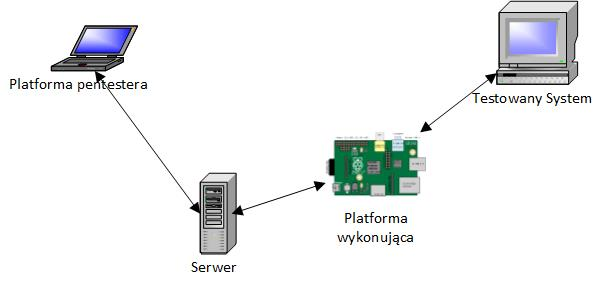
\includegraphics[width=\textwidth]{sprzet}
    \caption{Diagram komponentów sprzętowych}
    \label{fig:sprzet}
\end{figure}
\subsection[Wymagania funkcjonalne (Jakub Wyka)]{Wymagania funkcjonalne}
\begin{table}[H]
    \begin{tabular}{|p{2cm}|p{12cm}|}
        \hline
        \textbf{} & \textbf{Możliwość konfiguracji urządzenia testującego jako kartę sieciową} \\
        \hline
        Opis: & Możliwość konfiguracji platformy wykonującej, aby pełniła rolę i była wykrywana przez testowany system jako karta sieciowa. \\
        \hline
        Źródło: & Pentesterzy \\
        \hline
        Priorytet: & krytyczny \\ 
        \hline
    \end{tabular}  
    \label{tab:wym1}
\end{table}
%    \bigskip
\begin{table}[H]
    \begin{tabular}{|p{2cm}|p{12cm}|}
        \hline
        \textbf{} & \textbf{Możliwość konfiguracji urządzenia testującego jako klawiaturę} \\
        \hline
        Opis: & Możliwość konfiguracji platformy wykonującej, aby pełniła rolę i była wykrywana przez testowany system jako klawiatura. \\
        \hline
        Źródło: & Pentesterzy \\
        \hline
        Priorytet: & krytyczny \\ 
        \hline
    \end{tabular}  
    \label{tab:wym2}
\end{table}
%    \bigskip
\begin{table}[H]
    \begin{tabular}{|p{2cm}|p{12cm}|}
        \hline
        \textbf{} & \textbf{Możliwość wykonania testu zatruwania DNS} \\
        \hline
        Opis: & Możliwość wykonania testu bezpieczeństwa polegającego na podmianie rekordu DNS. \\
        \hline
        Źródło: & Pentesterzy \\
        \hline
        Priorytet: & krytyczny \\ 
        \hline
    \end{tabular}  
    \label{tab:wym3}
\end{table}
%    \bigskip
\begin{table}[H]
    \begin{tabular}{|p{2cm}|p{12cm}|}
        \hline
        \textbf{} & \textbf{Możliwość wykonania testu przechwytywania pakietów} \\
        \hline
        Opis: & Możliwość wykonania testu bezpieczeństwa polegającego na przechwyceniu pakietów. \\
        \hline
        Źródło: & Pentesterzy \\
        \hline
        Priorytet: & krytyczny \\ 
        \hline
    \end{tabular}  
    \label{tab:wym4}
\end{table}
    %\bigskip
\begin{table}[H]
    \begin{tabular}{|p{2cm}|p{12cm}|}
        \hline
        \textbf{} & \textbf{Możliwość wykonania testu przejęcia działania klawiatury} \\
        \hline
        Opis: & Możliwość wykonania testu bezpieczeństwa polegającego na przechwyceniu kontroli nad klawiaturą, a co za tym idzie nieograniczonych możliowości zaszkodzenia systemowi. \\
        \hline
        Źródło: & Pentesterzy \\
        \hline
        Priorytet: & krytyczny \\ 
        \hline
    \end{tabular}  
    \label{tab:wym5}
\end{table}
%    \bigskip
\begin{table}[H]
    \begin{tabular}{|p{2cm}|p{12cm}|}
        \hline
        \textbf{} & \textbf{Możliwość wyboru rodzaju testu z  poziomu serwera} \\
        \hline
        Opis: & Możliwość wyboru testu do przeprowadzenia z poziomu serwera. \\
        \hline
        Źródło: & Pentesterzy \\
        \hline
        Priorytet: & wysoki \\ 
        \hline
    \end{tabular}  
    \label{tab:wym6}
\end{table}    
%    \bigskip
\begin{table}[H]
    \begin{tabular}{|p{2cm}|p{12cm}|}
        \hline
        \textbf{} & \textbf{Zdalne uruchomienie testu} \\
        \hline
        Opis: & Możliwość rozpoczęcia wykonywania testu z poziomu serwera, który skomunikuje się z platformą testującą.\\
        \hline
        Źródło: & Pentesterzy \\
        \hline
        Priorytet: & wysoki \\ 
        \hline
    \end{tabular}  
    \label{tab:wym7}
\end{table}    
%   \bigskip
\begin{table}[H]
    \begin{tabular}{|p{2cm}|p{12cm}|}
        \hline
        \textbf{} & \textbf{Możliwość wyboru konkretnej platformy egzekucyjnej do przeprowadzenia testu} \\
        \hline
        Opis: & Możliwość wyboru konkretnej platformy egzekucyjnej, na której chcemy przeprowadzić test.\\
        \hline
        Źródło: & Pentesterzy \\
        \hline
        Priorytet: & wysoki \\ 
        \hline
    \end{tabular}  
    \label{tab:wym8}
\end{table}
%    \bigskip
\begin{table}[H]
    \begin{tabular}{|p{2cm}|p{12cm}|}
        \hline
        \textbf{} & \textbf{Możliwość kontroli testów za pomocą GUI na platformie pentestera} \\
        \hline
        Opis: & Możliwość użycia środowiska graficznego do kontroli wykonywania testów.\\
        \hline
        Źródło: & Pentesterzy \\
        \hline
        Priorytet: & średni \\ 
        \hline
    \end{tabular}  
    \label{tab:wym9}
\end{table}
%    \bigskip
\begin{table}[H]
    \begin{tabular}{|p{2cm}|p{12cm}|}
        \hline
        \textbf{} & \textbf{Możliwość raportowania wyników testu} \\
        \hline
        Opis: & Możliwość sporządzenia raportu z wykonania testu.\\
        \hline
        Źródło: & Pentesterzy \\
        \hline
        Priorytet: & krytyczny \\ 
        \hline
    \end{tabular}  
    \label{tab:wym10}
\end{table}
%    \bigskip
\begin{table}[H]
    \begin{tabular}{|p{2cm}|p{12cm}|}
        \hline
        \textbf{} & \textbf{Możliwość zdalnego raportowania wyników testu.} \\
        \hline
        Opis: & Możliwość przesłania sporządzonego raportu na serwer.\\
        \hline
        Źródło: & Pentesterzy \\
        \hline
        Priorytet: & wysoki \\ 
        \hline
    \end{tabular}  
    \label{tab:wym11}
\end{table}
%    \bigskip
\begin{table}[H]
    \begin{tabular}{|p{2cm}|p{12cm}|}
        \hline
        \textbf{} & \textbf{Możliwość przesłania rozkazu wykonania tego samego testu z danymi parametrami na kilka wybranych urządzeń testujących..} \\
        \hline
        Opis: & Możliwość jednoczesnego przesłania rozkazu wykonania tego samego testu z danymi parametrami na kilka wybranych urządzeń testujących..\\
        \hline
        Źródło: & Pentesterzy \\
        \hline
        Priorytet: & średni \\ 
        \hline
    \end{tabular}  
    \label{tab:wym12}
\end{table}
\subsection[Wymagania jakościowe (Jakub Wyka)]{Wymagania jakościowe}
\begin{table}[H]
\begin{tabular}{|p{2cm}|p{12cm}|}
    \hline
    \textbf{} & \textbf{Ochrona danych} \\
    \hline
    Opis: & Ochrona wszystkich danych przechowywanych przez system. \\
    \hline
    Źródło: & Zlecający testy penetracyjne \\
    \hline
    Priorytet: & krytyczny \\ 
    \hline
\end{tabular}  
\label{tab:wymf1}
\end{table}
%\vskip 0.3cm
\begin{table}[H]
\begin{tabular}{|p{2cm}|p{12cm}|}
    \hline
    \textbf{} & \textbf{Obsługa do 100 urządzeń wykonujących testy} \\
    \hline
    Opis: & Jednoczesna obsługa 100 urządzeń wykonujących testy. \\
    \hline
    Źródło: & Pentesterzy \\
    \hline
    Priorytet: & wysoki \\ 
    \hline
\end{tabular}  
\label{tab:wymf2}
\end{table}
%\vskip 0.3cm
\begin{table}[H]
\begin{tabular}{|p{2cm}|p{12cm}|}
    \hline
    \textbf{} & \textbf{Możliwość jednoczesnej pracy 10 pentesterów.} \\
    \hline
    Opis: & Możliwość jednoczesnego zarządzania systemem z 10 platform pentesterów na raz. \\
    \hline
    Źródło: & Pentesterzy \\
    \hline
    Priorytet: & wysoki \\ 
    \hline
\end{tabular}  
\label{tab:wymf3}
\end{table}
%\vskip 0.3cm
\begin{table}[H]
\begin{tabular}{|p{2cm}|p{12cm}|}
    \hline
    \textbf{} & \textbf{Uruchamianie GUI na dowolnej przeglądarce, systemie operacyjnym i platformie sprzętowej.} \\
    \hline
    Opis: & Możliwość uruchomienia GUI niezależnie od rodzaju platformy stosowanej przez pentestera. \\
    \hline
    Źródło: & Pentesterzy \\
    \hline
    Priorytet: & średni \\ 
    \hline
\end{tabular}  
\label{tab:wymf4}
\end{table}
%\vskip 0.3cm
\begin{table}[H]
\begin{tabular}{|p{2cm}|p{12cm}|}
    \hline
    \textbf{} & \textbf{Możliwość łatwego rozszerzenia funkcjonalności o kolejne scenariusze testowe.} \\
    \hline
    Opis: & Możliwość łatwego dodawania nowych scenariuszy testowych. \\
    \hline
    Źródło: & Pentesterzy \\
    \hline
    Priorytet: & średni \\ 
    \hline
\end{tabular}  
\label{tab:wymf5}
\end{table}
%\vskip 0.3cm
\begin{table}[H]
\begin{tabular}{|p{2cm}|p{12cm}|}
    \hline
    \textbf{} & \textbf{Czytelne raporty wykonanego testu.} \\
    \hline
    Opis: & Łatwe do analizy raporty z przeprowadzonych testów. \\
    \hline
    Źródło: & Pentesterzy \\
    \hline
    Priorytet: & średni \\ 
    \hline
\end{tabular}  
\label{tab:wymf6}
\end{table}
%\vskip 0.3cm
\begin{table}[H]
\begin{tabular}{|p{2cm}|p{12cm}|}
    \hline
    \textbf{} & \textbf{Zgodność ze standardami w zakresie GUI.} \\
    \hline
    Opis: & Wykorzystanie standardów w zakresie projektowania GUI pozwoli na intuicyjne korzystanie z systemu i skróci czas wdrożenia. \\
    \hline
    Źródło: & Pentesterzy \\
    \hline
    Priorytet: & średni \\ 
    \hline
\end{tabular}  
\label{tab:wymf7}
\end{table}
%\vskip 0.3cm
\begin{table}[H]
\begin{tabular}{|p{2cm}|p{12cm}|}
    \hline
    \textbf{} & \textbf{Wyświetlanie aktualnego stanu urządzenia Raspberry Pi Zero.} \\
    \hline
    Opis: & Wyświetlanie w dobrze widocznym miejscu informacji o aktualnym stanie urządzenia wykonującego. \\
    \hline
    Źródło: & Pentesterzy \\
    \hline
    Priorytet: & średni \\ 
    \hline
\end{tabular}  
\label{tab:wymf8}
\end{table}
%\vskip 0.3cm
\begin{table}[H]
\begin{tabular}{|p{2cm}|p{12cm}|}
    \hline
    \textbf{} & \textbf{Rozbudowany formularz parametryzacji testu.} \\
    \hline
    Opis: & Wybór parametrów testu przez specjalnie zaprojektowany formularz, aby niektóre z zadań mogły być przeprowadzone przez mniej wyszkolonych pracowników. \\
    \hline
    Źródło: & Pentesterzy \\
    \hline
    Priorytet: & średni \\ 
    \hline
\end{tabular}  
\label{tab:wymf9}
\end{table}
%\vskip 0.3cm
\begin{table}[H]
\begin{tabular}{|p{2cm}|p{12cm}|}
    \hline
    \textbf{} & \textbf{Możliwość samodzielnego wprowadzenia payloadu za pomocą pola tekstowego w gui.} \\
    \hline
    Opis: & Umożliwi to obsługę mniej standardowych wymagań klientów przez bardziej doświadczonych pracowników firmy. \\
    \hline
    Źródło: & Pentesterzy \\
    \hline
    Priorytet: & średni \\ 
    \hline
\end{tabular}  
\label{tab:wymf10}
\end{table}
\subsection[Wymagania sprzetowe(Jakub Wyka)]{Wymagania sprzetowe}

\begin{tabular}{|p{2cm}|p{12cm}|}
    \hline
    \textbf{} & \textbf{Konfiguracja serwera} \\
    \hline
    Opis: &  Min 2GB RAM \\
    &Procesor min. 2000 MHz
    \\
    \hline
    Źródło: & Pentesterzy \\
    \hline
    Priorytet: & krytyczny \\ 
    \hline
\end{tabular}  
\label{tab:wyms1}

\vskip 0.3cm

\begin{tabular}{|p{2cm}|p{12cm}|}
    \hline
    \textbf{} & \textbf{Konfiguracja urządzenia wykonującego} \\
    \hline
    Opis: 
    &  Nazwa: Raspberry Pi Zero \\
    &Procesor: Broadcom BCM2835 ARM11 (1 GHz)\\
    &  Pamięć RAM: 512 MB \\
    &  Złącza wideo: mini HDMI\\
    &  Łączność bezprzewodowa: WiFi 802.11 b/g/n, Bluetooth 4.0. \\
    &  Złącza: 1x micro USB OTG, 1x micro USB (tylko do zasilania) \\
    \hline
    Źródło: & Pentesterzy \\
    \hline
    Priorytet: & krytyczny \\ 
    \hline
\end{tabular}  
\label{tab:wyms2}

\vskip 0.3cm

\begin{tabular}{|p{2cm}|p{12cm}|}
    \hline
    \textbf{} & \textbf{Konfiguracja platformy Pentestera} \\
    \hline
    Opis: 
    &  Wymagania minimalne zgodne lub z wymaganiami najnowszej wersji Mozilla Firefox: \\
    &\begin{itemize}
        \item Pentium 4 albo nowszy procesor, który wspiera SSE2
        \item 512MB RAM / 2GB RAM dla 64-bit wersji
        \item 200MB przestrzeni dyskowej
    \end{itemize}
     \\
    \hline
    Źródło: & Pentesterzy \\
    \hline
    Priorytet: & krytyczny \\ 
    \hline
\end{tabular}  
\label{tab:wyms3}
\subsection[Wymagania jakościowe (Jakub Wyka)]{Wymagania programowe}

\begin{tabular}{|p{2cm}|p{12cm}|}
    \hline
    \textbf{} & \textbf{Wykorzystanie gotowego protokołu IOT do komunikacja między serwerem a urządzeniem testującym.} \\
    \hline
    Opis: & Wykorzystanie istniejącego protokołu komunikacyjnego. \\
    \hline
    Źródło: & pentesterzy \\
    \hline
    Priorytet: & wysoki \\ 
    \hline
\end{tabular}  
\label{tab:wymp1}

\vskip 0.3cm

\begin{tabular}{|p{2cm}|p{12cm}|}
    \hline
    \textbf{} & \textbf{Wykorzystanie istniejącego rozwiązania bazodanowego.} \\
    \hline
    Opis: & W celu łatwiejszego utrzymania produktu wymogiem jest użycie gotowego rozwiązania bazodanowego. \\
    \hline
    Źródło: & pentesterzy \\
    \hline
    Priorytet: & wysoki \\ 
    \hline
\end{tabular}  
\label{tab:wymp2}



\subsection[Diagram przypadków użycia]{Diagram przypadków użycia}

\begin{figure}[H]
    \centering
    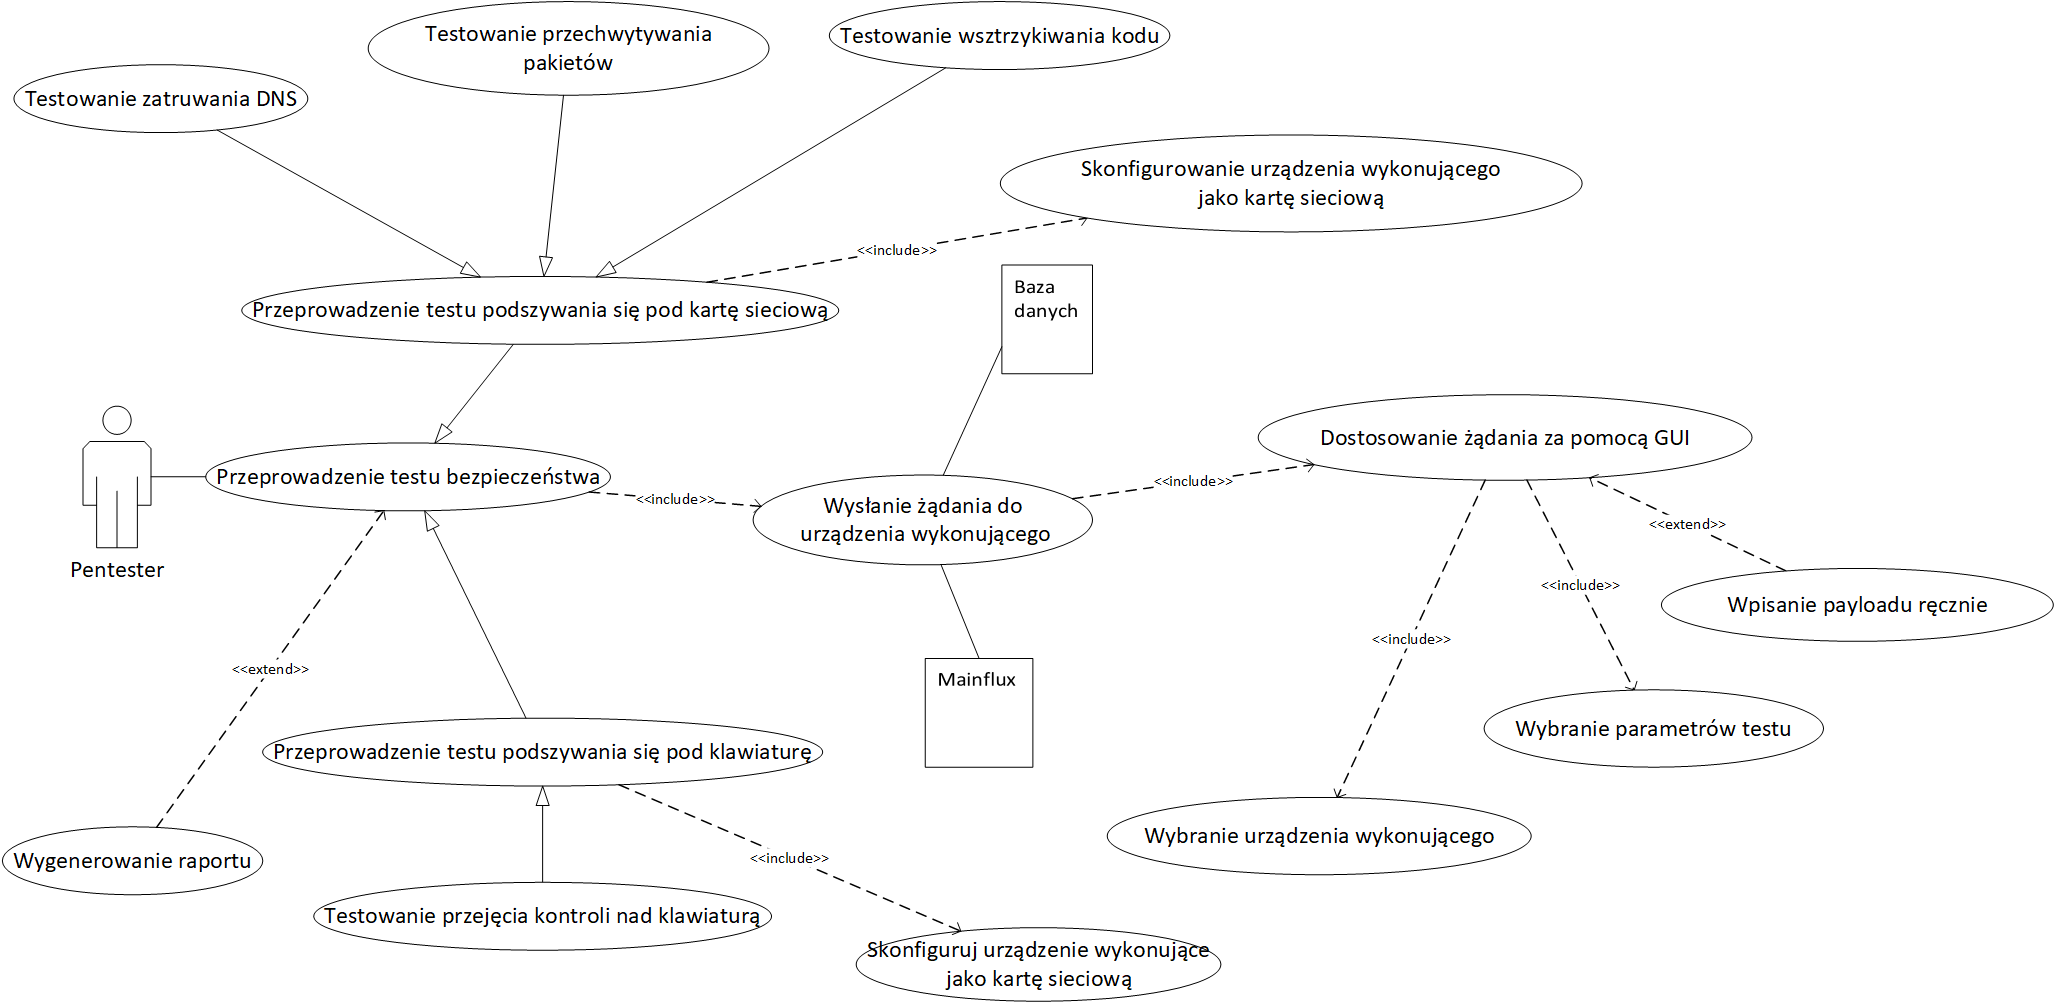
\includegraphics[width=\textwidth]{usecase}
    \caption{Diagram przypadków użycia}
    \label{fig:usecase}
\end{figure}
\subsection[Diagram klas]{Diagram klas}
\begin{figure}[H]
    \centering
    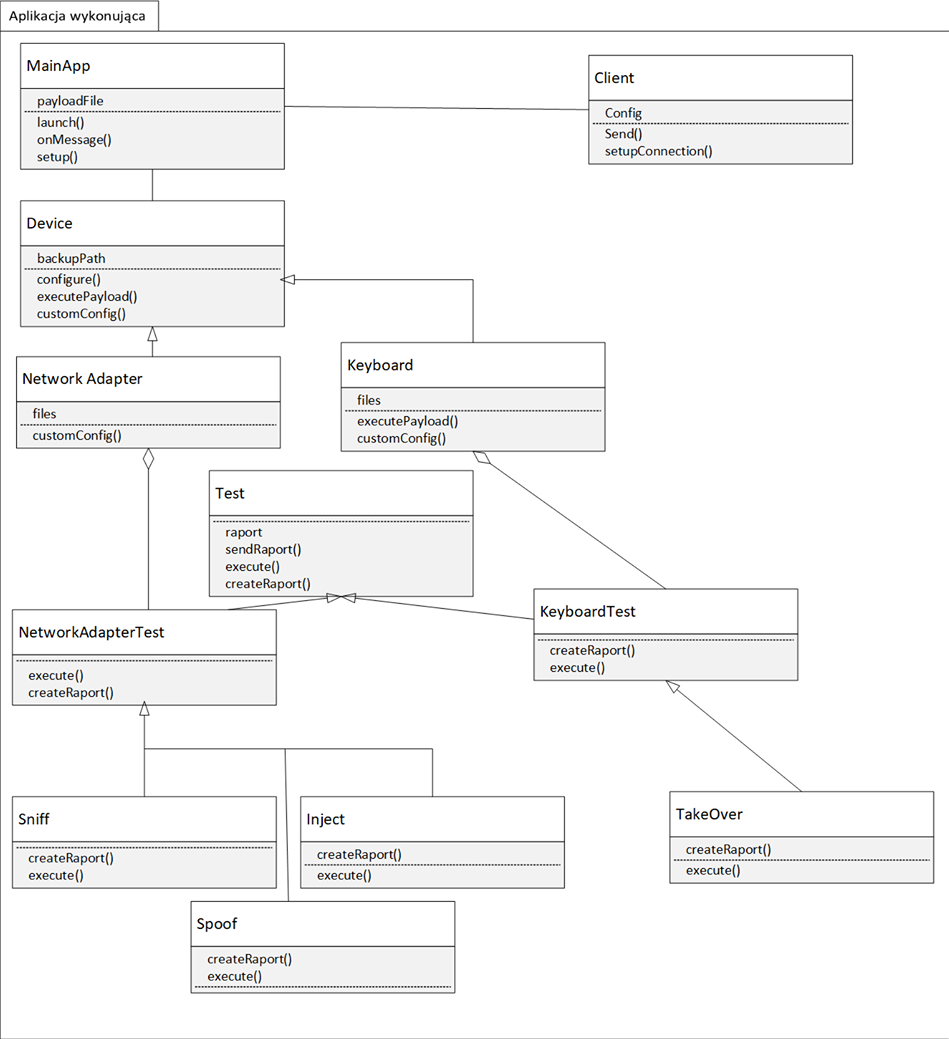
\includegraphics[width=\textwidth]{klaswyk}
    \caption{Diagram klas dot. aplikacji wykonującej}
    \label{fig:klaswyk}
\end{figure}

\begin{figure}[H]
    \centering
    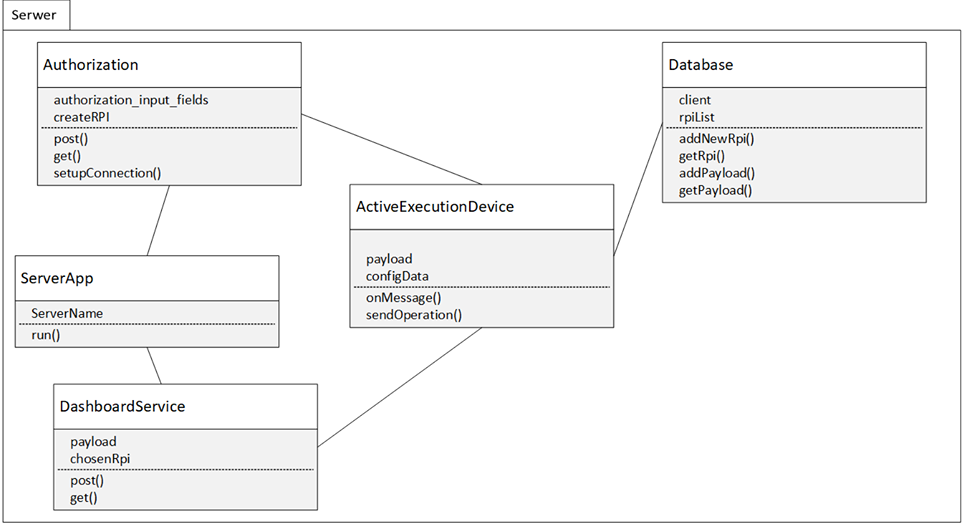
\includegraphics[width=\textwidth]{klasserw}
    \caption{Diagram klas dot. aplikacji serwerowej}
    \label{fig:klasserw}
\end{figure}

\begin{figure}[H]
    \centering
    \includegraphics[width=0.5\textwidth]{klasGUI}
    \caption{Diagram klas dot. interfejsu użytkownika}
    \label{fig:klasGUI}
\end{figure} \newpage
\section[Przygotowanie środowiska testowego (Kacper Połom)]{Przygotowanie środowiska testowego}
\label{chapter:enviroment}

\subsection[Cele]{Cele}
Głównym celem środowiska testowego jest ułatwienie oraz przyspieszenie pracy nad testowanym systemem. Pentester dzięki „środowisku ??” ma możliwość zdalnego zarządzania platformą wykonującą, która jest podpięta do testowanych urządzeń. Oznacza to, że z dowolnego miejsca może wysyłać komendy na każdą platformę wykonującą. To też znacznie przyspiesza badanie bezpieczeństwa, ponieważ pozwala na zautomatyzowane oraz równoczesne wykonywanie testów. 
Kolejnym celem takiego środowiska jest pokazanie aktywnych urządzeń, dzięki temu pentester wie, że wysłana komenda zostanie obsłużona. W przypadku braku wiedzy na ten temat czas pracy testera znacząco wzrósłby, ponieważ musiałby przy każdym wysyłaniu payloada upewniać się że platforma wykonująca otrzymała wiadomość. 
Dodatkowym atutem środowiska testowego jest automatyczne odbieranie wiadomości. Testy mogą wykonywać się przez dłuższy czas. W momencie, gdy tester wysyła payload na platformę nie musi czekać na odpowiedź.  Środowisko testowe automatycznie zapisze każdą przesłaną wiadomość oraz umożliwi późniejsze odczytanie. To pozwala na brak ciągłej aktywności pentestera oraz zabezpiecza przed utratą wiadomości, ponieważ tester może w każdym momencie sprawdzić przesłane informacje.
Zapewnienie dobrej komunikacji w środowisku testowym jest najważniejszym wymaganiem. Przy testowaniu nie można pozwolić sobie na jakąkolwiek utratę wiadomości. Podczas badania bezpieczeństwa, mogą być jednocześnie wysyłane wiadomości z różnych platform wykonujących na środowisko testowe jak i komendy z serwera na platforme to znaczy, że komunikacja musi być dwustronna. Dobrą komunikację, spełniającą wszystkie wymagania można uzyskać, przez użycie IoT.
Wyrażenie Internet Rzeczy pojawiło się już kilka lat temu i od tego czasu znacznie zyskało na popularności. Już teraz wiele firm oferuje nam różnie rozwiązania od termostatu do inteligentnych urządzeń domowych takie jak lodówka czy zmywarka.
Platforma IoT zapewnia łączność i normalizację, dzięki temu dane pobierane z różnych urządzeń, przy pomocy innych sposobów komunikacji, mają spójny format danych. Dodatkowym atutem jest zapewnienie bezpieczeństwa. Dane przesyłane z platformy wykonującej na środowisko testowe mogą mieć charakter danych szczególnie wrażliwych, dlatego ważnym jest żeby osoby trzecie nie miały do nich dostępu. Kolejną zaletą jest fakt, że przy IoT nie jest wymagana żadna interakcja pomiędzy człowiekiem a urządzeniem, co jest jednym z założeń przy tworzeniu środowiska testowego.
//coś dodać o autoryzacja??

\subsection[Przegląd platform IoT]{Przegląd platform IoT}
\label{subsection:platform}
Jest wiele platform IoT, które bardzo się różnią, dlatego przy szukaniu konkretnej warto przyjąć pewne założenie. Takim założeniem może być wybranie platformy, która nie zależy od hosta ani od jakości wsparcia, oznacza to, że taką platformę możemy uruchomić na dowolnej maszynie. Kolejnym założeniem jest wybranie platformy, która będzie darmowa, te warunki spełniają jedynie platformy z otwartym oprogramowaniem (ang. Open Sorce). Platformy IoT posiadają wiele różnic, mogą inaczej analizować dane (np. w czasie rzeczywistym, lub na prośbę użytkownika). Mogą również w inny sposób wizualizować zebrane dane, lub nie oferują wizualizacji. Takich różnic jest znacznie więcej, ale lepiej skupić się na najważniejszych aspektach, takich jak możliwość zarządzania platformami, obsługiwane protokoły umożliwiające zbieranie danych, język w jakim została napisana platforma, mechaniki do zapewnienia bezpieczeństwa oraz jakie bazy danych może obsłużyć platforma. 
\begin{table}[H]
    \begin{tabular}{|p{3cm}|p{2cm}|p{6.5cm}|p{1.5cm}|}
        \hline
        \textbf{Rodzaj platformy} & \textbf{Zarządzanie urządzeniami}  & \textbf{Protokoły do zbierania danych} & \textbf{Język} \\
        \hline
        Kaa IOT platform & tak & MQTT, CoAP, XMPP, TCP, HTTP & Java \\
        \hline
        Sitewhere  & tak & MQTT, AMQP, Stomp, WebSocket, DSC & Java \\
        \hline
        ThingSpeak & nie & HTTP & Ruby \\
        \hline
        Mainflux & tak & HTTP, MQTT, WebSocket, CoAP & Go \\
        \hline
        Zetta & nie & HTTP & Javascript \\
        \hline
    \end{tabular}
    \caption{Porównanie platform open sorce }  
    \label{tab:plat1}
\end{table}

\begin{table}[H]
    \begin{tabular}{|p{3cm}|p{6cm}|p{4.5cm}|}
        \hline
        \textbf{Rodzaj platformy} & \textbf{Bezpieczeństwo}  & \textbf{Obsługiwane bazy danych} \\
        \hline
        Kaa IOT platform & Ssl, RSA key 2048 & MongoDB, Cassandra, Hadoop, Oracle NoSQL \\
        \hline
        Sitewhere & Ssl, spring security & MongoDB, HBase , InfluxDB \\
        \hline
        ThingSpeak & Basic Authentication  & MySql \\
        \hline
        Mainflux & JWT encrypted, signed tokens, OAuth2.0, public key infrastructure (PKI) oraz client-side certificates & Cassandra, MongoDB, InfluxDB, PostgreSQL \\
        \hline
        Zetta  & Basic Authentication  & Brak \\
        \hline
    \end{tabular} 
    \caption{Porównanie platform open sorce} 
    \label{tab:plat2}
\end{table}
Zetta oraz ThingSpeak nie wspierają zarządzania urządzeniami oraz jedynym protokołem umożliwiającym przesyłanie danych jest HTTP. Ten protokół zapewnia wysoką gwarancję dostarczenia wiadomości oraz otrzymania odpowiedzi. Ma to jednak swoje minusy, ponieważ jego przepustowość jest znacznie mniejsza od MQTT. Komunikacja przy użyciu takiej technologii będzie zbyt wolna, szczególnie w momencie, gdy pentester będzie równocześnie testował wiele systemów. W odróżnieniu od tych dwóch platform Mainflux, SiteWhere oraz Kaa IoT wspierają protokoły, które są w stanie obsłużyć duży ruch, różnica pomiędzy nimi jest w zagwarantowaniu bezpieczeństwa. Mainflux pozwala na użycie Json Web Token (JWT). Jest to standard, który określa sposób bezpiecznego przesyłania wiadomości, jako obiekt JSON. Otrzymaną informację można zweryfikować, ponieważ jest podpisana cyfrowo. Taką wiadomość można podpisać z użyciem klucza tajnego (algorytm HMAC) albo za pomocą pary kluczy publiczny / prywatny (algorytm RSA lub ECDSA). Dodatkowo te trzy platformy używają dockera co pozwala na szybkie uruchamianie oraz łatwą dystrybucję. %Docker jest to narzędzie pozwalające na łatwiejsze tworzenie, wdrażanie oraz uruchamianie aplikacji. Umożliwia również korzystanie z tego samego jądra Linuksa, co system, na którym działa. Daje to wysoki wzrost wydajności, oraz zmniejsza rozmiar.
Atutem Mainfluxa jest język w jakim został napisany, dzięki Go rozmiar kontenera jest niewielki, poza tym kod napisany w takim języku jest znacznie szybszy od tych w Javie czy C\#, wynika to z faktu, że Go jest językiem kompilowanym. Kolejną zaletą jest fakt, że język Go jest stosunkowo młody oraz ciągle rozwijany przez firmę Google. Dzięki wsparciu dużej korporacji oraz ciągle rosnącej popularności, można mieć pewność, że ten język będzie stawał się coraz lepszy. %//może jeszcze 2 słowa co nam daje fakt że jęzk go jest ciągle rozwijany???
Platforma Mainflux wydaje się być najlepszym wyborem przy tworzeniu ST. Przewagę nad innymi platformami zawdzięcza wykorzystywanym technologiom oraz bezpieczeństwu. Oferuje wiele rozwiązań ochrony przesyłanych informacji.
Silne strony Mainfluxa to także dokumentacja~\cite{mainflux} oraz wysoka swoboda sposobu implementacji, pozwalająca lepiej dopasować platformę do własnych potrzeb.
%bardzo dobrej dokumentacji. 
%Mainflux również się wyróżnia pod względem 

\subsection[Mainflux]{Wybrana platforma}
Mainflux umożliwia połączenie urządzeń do aplikacji oraz jednocześnie poprzez wykorzystanie JWT zapewnia bezpieczeństwo na wysokim poziomie. Tak jak zostało przedstawione w tabeli~\ref{tab:plat1}, mainflux oferuje wieloprotokołowy przekaźnik komunikatów, pozwala to na wybranie odpowiedniego protokołu do zapewnienia niezbędnych wymagań.
Mainflux jest używany jako oprogramowanie pośrednie to oznacza, że wykorzystuje serwer, który udostępnia funkcje oraz usługi potrzebne do stworzenia aplikacji IoT. Podstawowymi usługami są: 


\begin{itemize}
    \item Messaging bridge pośredniczy w wysyłaniu wiadomości pomiędzy urządzeniem a aplikacją. 
    \item User manager (Mainflux UI, Mainflux CLI) – umożliwia użytkownikowi zarządzanie zasobami. Pierwszy sposób to zarządzanie przez stronę internetową (Mainflux UI). Aby użytkownik mógł zarządzać zasobami musi się zalogować na stronie, po czym ma możliwość dodawania, usuwania, edycji rzeczy oraz łączenia kanałów z rzeczami. Drugim sposobem jest bootstraping (Mainflux CLI) czyli zautomatyzowane zarządzanie zasobami, wykorzystując bootstraping rejestracja nowych urządzeń może odbywać się bez udziału człowieka.
    \item Normalizer służy do zmieniania struktury wiadomości. Mainflux może otrzymywać wiadomości, w różnych formatach. Normalizer zmienia przesłaną wiadomość na format SenML (Sensor Markup Language), po czym przekazuje ją do zapisania w bazie danych.
    \item NATS otrzymuje wiadomości od rzeczy i może automatycznie reagować na przesłane dane, w oparci o konfigurowalny zestaw reguł.
    \item Writer służy do zapisywania komunikatów w bazie danych. Ponieważ istnieje wiele różnych systemów baz danych, dla każdego z nich musi istnieć odpowiedni moduł piszący​.
\end{itemize}

Poniższy schemat pokazuje zależności między tymi usługami.

\begin{figure}[H]
    \centering
    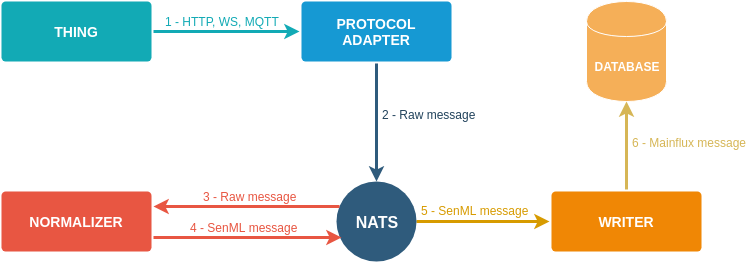
\includegraphics[width=\textwidth]{kp03}
    \caption{Placeholder}
    \label{fig:iotarch}
\end{figure}
//https://medium.com/mainflux-iot-platform/mainflux-open-source-iot-platform-set-up-and-usage-70bed698791a pozniej dodam do zrodel 

Aby zrozumieć jak działa przesyłanie wiadomości za pośrednictwem platformy mainflux trzeba poznać trzy podstawowe koncepty jakie zostały wprowadzone.
\begin{itemize}
    \item Użytkownik reprezentuje człowieka w systemie, który jest identyfikowany za pomocą danych do logowania jest on używany do zarządzania innymi zasobami. Zarządzanie obejmuje tworzenie, edytowanie oraz usuwanie rzeczy  i kanałów, a także do łączenia rzeczy z kanałami. 
    \item Rzecz reprezentuje urządzenie lub aplikację każda rzecz posiada identyfikator oraz klucz dodatkowo, może mieć przypisany typ (aplikacja, urządzenie). 
    \item Kanał pozwala na połączenia rzeczy między sobą. Każdy kanał ma swoje id, do kanału może być podłączonych więcej niż 2 rzeczy, każdy kto nasłuchuje na danym kanale otrzymuje tą wiadomość.
\end{itemize}


\subsection[Przegląd protokołów wykorzystywanych w IoT]{Przegląd protokołów wykorzystywanych w IoT}
Do realizacji ST zdecydowano się wykorzystać rozwiązania IoT. Kluczową decyzją projektową dla tej części systemu będzie wybranie platformy~\ref{subsection:platform}.
Wiedza o wykorzystywanych przez nie protokołach pozwoli dokonać lepszego wyboru. Informację na temat wykorzystywanych protokołach w IoT można znaleźć w takim artykule~\cite{porownanie_protokolow}. W rozwiązaniach IoT popularne są protokoły:
\begin{itemize}
    \item Message Queue Telemetry Transport (MQTT) jest lekkim protokołem transmisji danych, umożliwia komunikację między urządzeniami za pośrednictwem serwera. MQTT jest oparty o wzorzec Publish-Subscribe, wzorzec ten mówi, że wiadomość od nadawcy nie trafia bezpośrednio do odbiorcy tylko najpierw trafia do serwera pośredniczącego (ang. broker). Dzięki serwerowi pośredniczącemu odbiorca nic nie wie o osobie która nadaje wiadomość oraz nie dostaje potwierdzenia o doręczonej wiadomości. %//tutaj trzebaz zmienić jeśli dodam Qos.
    Plusami protokołu MQTT jest na pewno prędkość przesyłania danych, zawdzięcza to dzięki małemu narzutowi na transportowane dane. Narzut na dane oznacza, ile jest potrzebnych dodatkowych bajtów przy wysłaniu wiadomości, najmniejszy pakiet (przy zastosowaniu MQTT) ma tylko dwa bajty metadanych~\cite{protokol_mqtt}. Jest to również protokół binarny, co wpływa na zmniejszenie obciążenia. Dodatkowo zapewnia bardzo wysoką niezawodność transmisji, dlatego idealnie sprawdza się przy połączeniach między dwoma urządzeniami. Kolejną zaletą protokołu MQTT jest możliwość komunikacji dwukierunkowej oznacza to, że klient MQTT może być równocześnie subskrybentem jak i publisherem. %// można jeszcze dodać coś o możliwość zarządzania jakością usług ale tego nie robiliśmy więc nwm czy wspominać ??
\end{itemize}
\begin{figure}[H]
    \centering
    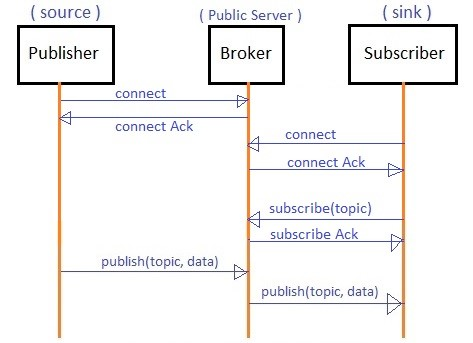
\includegraphics[width=\textwidth]{kp07}
    \caption{Diagram przesyłania wiadomości w protokole MQTT} %publish/subscribe
    \label{fig:iotarch1}
\end{figure}
\begin{itemize}
    \item WebSocket jest protokołem opartym na TCP, tak jak MQTT zapewnia komunikację dwukierunkową. Po zestawieniu połączenia zarówno serwer jak i urządzenie mogą w dowolnym momencie wymieniać się danymi. WebSocket jest dużo lepszym rozwiązaniem od np. AJAX long polling (rozwiązanie, gdzie klient wysyła żądanie a serwer odpowiada), ponieważ mogą obsłużyć w tym samym czasie większą ilość zapytań. Minusem tego rozwiązania jest duży narzut danych, wynikający z złożoności ramek.
\end{itemize}
\begin{figure}[H]
    \centering
    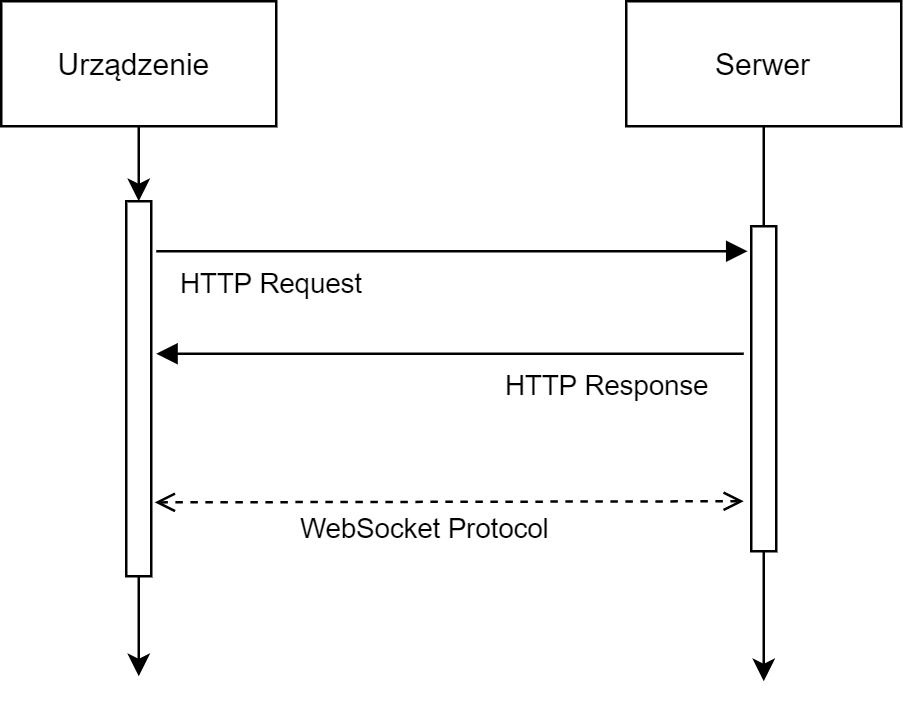
\includegraphics[width=\textwidth]{kp05}
    \caption{Diagram ukazujący jak działa Websocket}
    \label{fig:iotarch2}
\end{figure}
\begin{itemize}
    \item Constrained Application Protocol (CoAP) to protokół warstwy aplikacji, który jest stosowany do urządzeń z ograniczonymi zasobami. CoAP jest oparty na UDP a nie TCP, dlatego klient komunikuje się z serwerem bezpołączeniowo. Umożliwia również komunikowanie się za pomocą podobnych protokołów oraz obsługuje multiemisjie. CoAP został zaprojektowany do komunikacji między urządzeniami znajdującymi się w tej samej ograniczonej sieci.
\end{itemize}
\begin{figure}[H]
    \centering
    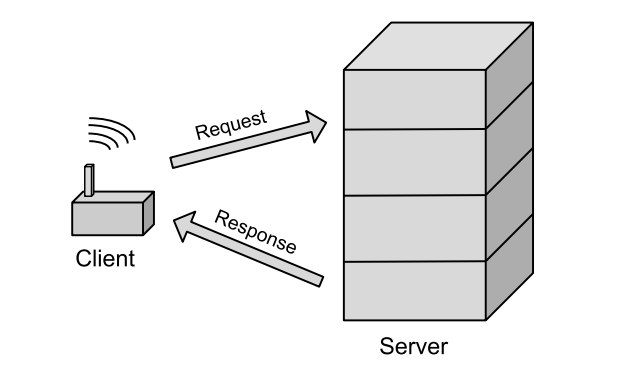
\includegraphics[width=\textwidth]{kp06.png}
    \caption{Schemat pokazujący sposób komunikacji w protokole CoAP}
    \label{fig:iotarch3}
\end{figure}
\begin{itemize}
    \item Hypertext Transfer Protocol (HTTP) to protokół warstwy aplikacji, który służy do przesyłania dokumentów hipermedialnych. HTTP jest oparty o wzorzec klient-serwer, gdzie klient (lub serwer proxy w jego imieniu) wysyła żądanie, a następnie czeka na odpowiedz. Protokół HTTP jest bezstanowy, oznacza to, że nie zawiera żadnych danych o połączeniu. Najczęściej jest oparty na warstwie TCP / IP, może być również na dowolnej niezawodnej warstwie transportowej.
\end{itemize}
\begin{figure}[H]
    \centering
    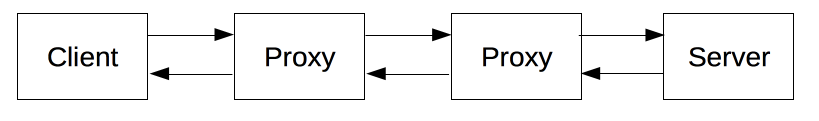
\includegraphics[width=\textwidth]{kp08.png}
    \caption{Wykorzystanie serwerów proxy w komunikacji}
    \label{fig:iotarch4}
\end{figure}
%W kolejnym podrozdziale zostaną porównane platformy IoT, między innymi pod względem obsługiwanych protokołów. Ważnym jest, żeby platforma mogła przesyłać dane za pośrednictwem protokołu MQTT.
%Głównie przez fakt, że w porównaniu do innych rozwiązań oferuje znacznie szybszy przekaz wiadomości oraz większą przepustowość.
\subsection[Architektura]{Architektura}
\begin{figure}[H]
    \centering
    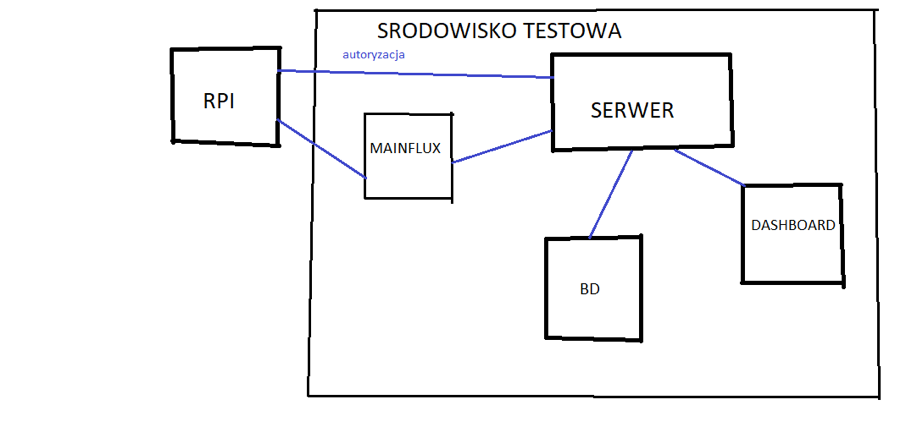
\includegraphics[width=\textwidth]{kp01}
    \caption{Schemat przedstawiający podstawowe zależności w środowisku testowym } % role Środowiska testowego w dedykowanym systemie
    \label{fig:iotarch}
\end{figure} 
Serwer ma kilka zadań do spełnienia, pierwszym jest zapewnienie autoryzacji platformy wykonującej. Każda platforma ma swój zewnętrzny identyfikator oraz klucz, w momencie, gdy platforma wykonująca chce otrzymać swoje dane (tzn. klucz rzeczy, identyfikator rzeczy oraz 2 przypisane kanały) wysyła żądanie HTTP na serwer z zewnętrznym identyfikatorem oraz kluczem. Platforma wykonująca potrzebuje 2 kanały, ponieważ na jednym będzie wysyłała wiadomości, a na drugim odbierał. Serwer po otrzymaniu zapytania sprawdza czy zewnętrzny identyfikator przesłany przez platformę wykonującą znajduję się już w bazie danych, jeśli tak to pobiera jego dane oraz zwraca je. W przeciwnym razie serwer dzięki Mainflux-cli loguje się jako administrator, tworzy nową rzecz oraz 2 kanały, po czym przypisuje je do stworzonej rzeczy oraz do rzeczy serwera. Rzecz serwera jest to utworzony obiekt przy starcie środowiska testowego, który ma przypisane do siebie wszystkie kanały. 
Kolejnym zadaniem serwera jest przesyłanie wiadomości z panelu użytkownika na platformę wykonującą oraz odbieranie wiadomości od platformy wykonującej. Wysyłanie wiadomości jest stosunkowo łatwe. Wystarczy, że serwer wyśle payload na odpowiedni kanał, który nasłuchuje w tym samym czasie. Z kolei odbieranie wiadomości jest bardziej skomplikowane, aby odebrać wiadomość serwer musi nasłuchiwać na kanale. Ze względu na to, że wiele platform wykonujących może w tym samym momencie wysyłać wiadomości, środowisko testowe powinno jednocześnie nasłuchiwać na wszystkich kanałach. Serwer dodaje kanały które znajdują się w bazie danych. Oznacza to, że w momencie gdy nowa platforma wykonująca przechodzi proces autoryzacji, serwer musi automatycznie odświeżyć listę kanałów, które nasłuchują na przesłaną wiadomości.
Środowisko oferuje rest api, które pozwoli na udostępnienie metod potrzebnych do stworzenia Dashboardu. Dashboard jest to łatwy w odczycie interfejs, który pośredniczy miedzy pentesterem a serwerem. Jednym z celów rest api jest umożliwienie pobrania wiadomości, jakie serwer odebrał. Pozwala to pentesterowi na przeglądanie wiadomości. Kolejna metoda ma za zadanie zwrócić listę aktywnych platform wykonujących. Ta lista znajduje się na serwerze oraz jest uaktualniana co 5 sekund. Uaktualnianie polega na tym, że platforma wykonująca co 2s zgłasza aktywność, jeśli serwer nie otrzyma wiadomości od platformy przez więcej niż 4s aktualny wynik zostaje usunięty. Następną udostępnioną metodą jest wysłanie ładunku na platformę wykonującą. Serwer pozwala na wysłanie wiadomości na wskazaną platformę lub do wszystkich aktywnych urządzeń. Aby pentester mógł wysłać payload na pojedynczą platformę, musi wpisać zewnętrzny identyfikator urządzenia. Serwer, który otrzyma zapytanie z takim identyfikatorem sprawdza, czy wskazane urządzenie istnieje, jeśli tak to pobiera jego kanał, na którym nasłuchuje oraz wysyła wiadomość. Odpowiedź pentester będzie mógł przeczytać na liście przesłanych wiadomości.
%/rysunek Thing – channel – thing może coś jeszcze o plusch wysyłania na wszystkie platformy Odseparowanie interfejsu użytkownika od operacji na serwerze.
\subsection[Problemy]{Problemy}
\begin{itemize}
    \item CORS
    \item OPÓŹNIENIE WYSYŁANIA WIELU WIADOMOŚCI (SLEAP(0.0001))
    \item Po 2 kanały do każdego  urządzenia //być może o tym w pkt. 5
    \item Używana technologia (python, swagger, flask, paho)
\end{itemize}
 \newpage
\section[Symulowanie działania klawiatury USB (Michał Krakowiak)]{Symulowanie działania klawiatury USB}
\label{chapter:usbkeyboard}
Realizacja projektu zakładała implementację symulowania działania klawiatury USB. W tym rozdziale zostaną omówione najważniejsze aspekty dotyczące realizacji tej funkcjonalności. 

\subsection[Scenariusz (Kacper Połom)]{Scenariusz} \label{sce:klawiatura}
Test polega na zdalnym wprowadzeniu dowolnej sekwencji klawiszy w systemie komputerowym. Oczekiwanym rezultatem jest odebranie danych przez system w taki sposób jakby wprowadzał je faktyczny użytkownik.
\subsubsection[Aktorzy]{Aktorzy}
\begin{itemize}
    \item Pentester - osoba przeprowadzająca test bezpieczeństwa systemu komputerowego za pomocą dedykowanego systemu
    \item Serwer sterujący - centralny punkt infrastruktury, który opowiada na zapytanie od testowanego systemu
    \item Urządzenie wykonujące - niewielkie urządzenie oparte o platformę Raspberry Pi Zero W, podłączone za pomocą portu USB do testowanego systemu
    \item Testowany system - system komputerowy pracujący pod kontrolą systemu \textit{Windows 10}, użytkownik nie posiada uprawnień administratora
\end{itemize}
\subsubsection[Założenia początkowe]{Założenia początkowe}
Prawidłowa realizacja scenariusza wymaga, aby urządzenie wykonujące było podłączone przez port USB do testowanego systemu. Powinno ono posiadać własne połączenie z internetem. Testowany system komputerowy musi być włączony, żeby mógł dostarczyć zasilanie urządzeniu oraz odebrać od niego dane.
\subsubsection[Przebieg]{Przebieg}
Urządzenie wykonujące po otrzymaniu zasilania uruchamia skrypt, który odpowiada za komunikację z serwerem i obsługę komunikacji przy użyciu USB.
Urządzenie rejestruje swoją obecność na serwerze sterującym.
Pentester przy pomocy dedykowanego panelu wskazuje urządzenie oraz wysyła do niego ładunek - wskazaną sekwencję klawiszy.
Serwer rozróżnia testowane systemy na podstawie zgłoszonych identyfikatorów. W tym samym czasie może być testowanych wiele systemów komputerowych.
Po otrzymaniu wiadomości z ładunkiem urządzenie wykonujące realizuje komunikację przez port USB i wysyła informacje o wciśnięciu kolejnych klawiszy. Przykładowym efektem takich działań może być uruchomienie wiersza poleceń oraz wprowadzenie skryptu powłoki, co można zaklasyfikować jako zdalne wykonanie kodu. Odstępy czasowe pomiędzy symulowaniem wciśnięcia kolejnych klawiszy są na tyle małe, że proces jest praktycznie niezauważalny dla użytkownika.
\begin{figure}[H]
    \centering
    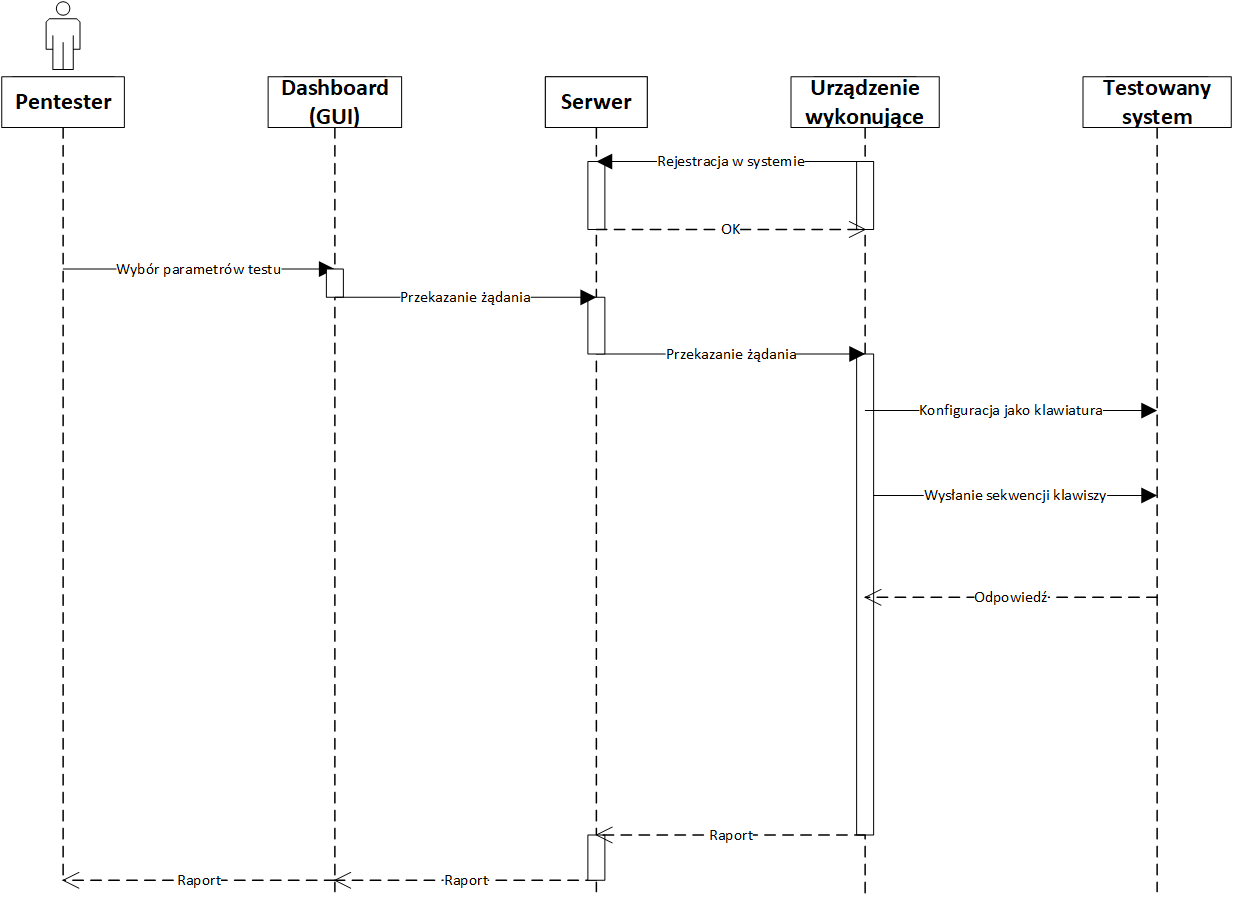
\includegraphics[width=\textwidth]{intKlaw}
    \caption{Diagram interakcji dot. testu symulowania działania klawiatury}
    \label{fig:klawiatura}  
\end{figure}
\subsection[Ogólny mechanizm działania (Michał Krakowiak)]{Ogólny mechanizm działania}
\label{chapter:keyboard_mechanics}
Podłączenie urządzenia wykonującego do testowanego systemu powinno skutkować rozpoznaniem go jako tzw. Human Interface Device, dalej określanego jako HID. HID to klasa urządzeń korzystających z interfejsu USB do interakcji z człowiekiem, czyli użytkownikiem komputera.
Zazwyczaj wykorzystywane są do pobierania danych wejściowych~\cite{oney}. Interfejs jest powszechnie stosowany przez producentów akcesoriów oraz dobrze udokumentowany w specyfikacji USB~\cite{usbhid}.
Dzięki wysokiej adopcji standardu popularne systemy takie jak Windows, Linux czy macOS są w stanie automatycznie identyfikować nowe urządzenia i korzystać z ich podstawowych funkcjonalności. Często nie ma potrzeby instalacji dedykowanych sterowników.
Ułatwia to pracę pentestera korzystającego z realizowanego systemu. Jeżeli nie planuje on przygotowania niestandardowej funkcjonalności to nie musi implementować i dostarczać własnych sterowników na każdy testowany system komputerowy.
Urządzenia HID komunikują się z komputerem po przez blok danych nazywany raportem. Bity i bajty w nim sformatowane są w sposób określony w deskryptorze raportu.
Listing~\ref{lst:desc} stanowi fragment deskryptora odczytanego bezpośrednio z rzeczywistej klawiatury.
\begin{lstlisting}[language={},label={lst:desc},caption={Przykładowy deskryptor odczytany z istniejącej klawiatury}]
Usage Page (Desktop),                   ; Generic desktop controls (01h)
Usage (Keyboard),                       ; Keyboard (06h, application collection)
Collection (Application),
    Usage Page (Keyboard),              ; Keyboard/keypad (07h)
    Usage Minimum (KB Leftcontrol),     ; Keyboard left control (E0h, dynamic value)
    Usage Maximum (KB Right GUI),       ; Keyboard right GUI (E7h, dynamic value)
    Logical Minimum (0),
    Logical Maximum (1),
    Report Size (1),
    Report Count (8),
    Input (Variable),
    Report Count (1),
    Report Size (8),
    Input (Constant),
    Report Count (3),
    Report Size (1),
    Usage Page (LED),                   ; LEDs (08h)
    Usage Minimum (01h),
    Usage Maximum (03h),
    Output (Variable),
    Report Count (5),
    Report Size (1),
    Output (Constant),
    Report Count (6),
    Report Size (8),
    Logical Minimum (0),
    Logical Maximum (255),
    Usage Page (Keyboard),              ; Keyboard/keypad (07h)
    Usage Minimum (None),               ; No event (00h, selector)
    Usage Maximum (FFh),
    Input,
End Collection
\end{lstlisting}
Każdy deskryptor rozpoczyna się od dyrektywy \textit{Usage Page},
która wskazuje interpretacje kolejnych stałych liczbowych.
Dostępne są tabele zawierające wszystkie możliwe wartości pól deskryptora.
Są one dostarczane przez twórców standardu jako \textit{HID Usage Tables}~\cite{hut}.
Pole \textit{Collection} opisuje zbiór powiązanych ze sobą elementów. W tym przypadku są to raporty: wyjściowy i wejściowy.
Raport wejściowy \textit{(ang. input report)} jest przekazywany do systemu komputerowego i zawiera informację o wciśniętych klawiszach.
Z kolei raport wyjściowy \textit{(ang. output report)} jest przeznaczony dla urządzenia USB i może być wykorzystywany np. do ustawiania jego stanu.
Ważny odnotowania jest fakt, że opisy pól w raportach mogą być wymieszane ze sobą.
Człowiek może mylnie interpretować obecność w sumie 5 dyrektyw \textit{Input} i \textit{Output} jako opis 5 różnych struktur.
W rzeczywistości należy je odczytywać jako przynależność do poszczególnych typów.
Z deskryptora przytoczonego listingu~\ref{lst:desc} można odczytać struktury składające się z:
\begin{itemize}
    \item 8 jednobitowych pól raportu wejściowego, każe przyjmuje wartości od 0 do 1. Poszczególne bity odpowiadają modyfikatorom takim jak np. shift lub alt.
    \item 1 ośmiobitowe pole raportu wejściowego o stałej wartości, to pole nie wpływa na interpretację danych, więc dalszy opis można pominąć
    \item 3 jednobitowe pola raportu wyjściowego, które odpowiadają za modyfikatory diód LED klawiatury (np. wskaźnik caps lock)
    \item 5 jednobitowych pól raportu wyjściowego o stałej wartości, stanowią dopełnienie do pojedyńczego bajtu
    \item 6 ośmiobitowych pól raportu wejściowego o wartościach od 0 do 255, odpowiadają kodom wciśniętych klawiszy
\end{itemize}
Wynikowe struktury ilustruje rysunek~\ref{fig:report}.
%TODO ogarnąć grafikę odpowiadającą deskryptorowi
\begin{figure}[H]
    \centering
    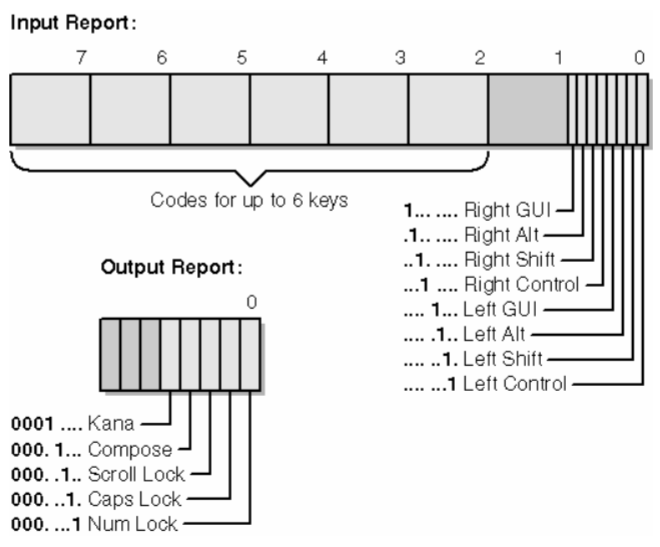
\includegraphics[width=\textwidth]{images/mk02.png}
    \caption{Struktura raportu~\cite{oney}}
    \label{fig:report}
\end{figure}
Implementacja symulowania działania klawiatury będzie polegała na implementacji generowania prawidłowych raportów wejściowych.
Obsługę raportów wejściowe można zignorować. Nie jest ona wymagana do poprawnego działania systemu, ponieważ zapalanie odpowiednich indykatorów nie jest częścią wymagań funkcjonalnych.
Wartości, jakie należy nadać poszczególnym bajtom, aby wskazać wciśnięcie danego klawisza można odczytać z przytoczonego już \textit{HID Usage Tables}. 
Warto mieć na uwadze, że nie ma żadnego powiązania z kodami ASCII. Przykładowo wartość zarówno dla znaków 'a' oraz 'A' to 04h (rozróżnia je odpowiedni modyfikator przesyłany w pierwszym bajcie), podczas gdy w ASCII to odpowiednio 61h i 41h. Obsługa kodu klawisza wysyłane przez urządzenia HID może się różnić w zależności od systemu operacyjnego, np. tylko system MacOS obsługuje kody klawiszy od F13 do F15~\cite{hut}.

\subsection[Konfiguracja]{Konfiguracja}
Do skonfigurowania urządzenia wykonującego jako kartę sieciową wykorzystujemy wsparcie platformy dla \textit{usb gadget modes}. Jest to możliwe dzięki złączu Universal Serial Bus (USB) znajdującemu się na płytce Raspberry Pi Zero mogącemu pracować w trybie \textit{On-The-Go} (OTG). Oznacza to, że urządzenie może zmieniać swoją rolę pomiędzy \textit{host} i \textit{slave}. W przypadku działania urządzenia jako karta sieciowa potrzebny jest tryb \textit{slave}, który nazywany jest też \textit{device}. Konieczne są również odpowiednie moduły jądra systemu Linux dostarczone przez system \textit{Raspbian}, które za pomocą odpowiedniej konfiguracji zostają załadowane do systemu. W zależności, który z nich zostanie wybrany realizowana będzie inna funkcjonalność. W tym przypadku jest to g\_ether - ethernet gadget driver oraz dwc2 - sterownik zajmujący się obsługą funkcjonalności USB OTG.
Po załadowaniu wyżej wymienionych modułów możliwe jest korzystanie z interfejsu \textit{usb0}, jednak trzeba go skonfigurować. Nadajemy statyczny adres IP aby możliwe było późniejsze jednoznaczne odwoływanie się do niego (patrz listing~\ref{lst:ifconfig}).
\begin{lstlisting}[language=bash,caption={Konfiguracja interfejsu \textit{usb0}},label={lst:ifconfig}]
    ifconfig usb0 192.168.100.1 netmask 255.255.255.0 up
\end{lstlisting}
W celu automatycznej konfiguracji hosta z pomocą DHCP zastosowano serwer \textit{Dnsmasq}. Pozwala to na automatyczne przypisanie adresu IP do interfejsu,
do którego podpięty został kabel USB w testowanym komputerze. Do poprawnego działania serwera konieczne jest edytowanie pliku konfiguracyjnego \textit{/etc/dnsmasq.conf}.
Należy ustawić interfejs oraz adres IP, na którym nasłuchiwać mają usługi DHCP i DNS oraz pulę adresów IP (patrz listing~\ref{lst:dhcp}).\newpage
\begin{lstlisting}[language=bash,caption={Konfiguracja serwera DHCP},label={lst:dhcp}]
    interface=usb0
    listen-address=192.168.100.1
    dhcp-range=192.168.100.50,192.168.100.150,12h 
\end{lstlisting}
Następnie należy włączyć \textit{IP forwarding}, aby możliwe było przekazywanie pakietów pomiędzy interfejsami \textit{usb0} oraz \textit{wlan0}.
Konfigurujemy je za pomocą polecenia iptables, w którym określamy reguły przepływu pakietów (patrz listing~\ref{lst:iptables}). 
\begin{lstlisting}[language=bash,caption={Ustawianie reguł przepływu pakietów},label={lst:iptables}]
    iptables -t nat -A POSTROUTING -o wlan0 -j MASQUERADE
    iptables -A FORWARD -i wlan0 -o usb0 -m state --state RELATED,ESTABLISHED -j ACCEPT
    iptables -A FORWARD -i usb0 -o wlan0 -j ACCEPT 
\end{lstlisting}
\begin{enumerate}
    \item Wszystkie pakiety opuszczające urządzenie przez interfejs \textit{wlan0}, są poddawane operacji maskarady, która poprawia bezpieczeństwo ukrywając wewnętrzne adresy IP w danej sieci.
    \item Akceptacja przekazywania pakietów z interfejsu \textit{wlan0} do interfejsu \textit{usb0}
    \item Akceptacja przekazywania pakietów z interfejsu \textit{usb0} do interfejsu \textit{wlan0}
\end{enumerate}

%\subsection[Wysyłanie sekwencji klawiszy (Michał Krakowiak)]{Wysyłanie sekwencji klawiszy}
Komentarz: korzystamy z HID do wysyłania kodów klawiszy, standard dosyć dokładnie opisuje co i jak, może tabele z dokumentacji?
Czym jest report (HID)
Czym jest deskryptor (HID)
HID też nie kojarzę, żeby był omawiany szerzej – potencjalne miejsce do rozpisania, niestety aktualnie zabrakło czasu
Po zakończeniu konfiguracji urządzenie wykonujące jest gotowe do podłączenia do systemu komputerowego, który ma zostać poddany testowi penetracyjnemu. Urządzenie po otrzymaniu zasilania z portu USB, zostanie wykryte przez system operacyjny jako klawiatura. 

\subsection[Wykrywalnosc (Jakub Wyka)]{Wykrywalność złośliwego urządzenia USB w konfiguracji karty sieciowej}
\label{subsec:wykrywalnoscJW}

W systemie \textit{Windows} podczas konfiguracji urządzenia pojawia się okienko systemowe opisane wcześniej w
 sekcji~\ref{subsec:wykrywalnoscMK}. Poza nim, po udanej konfiguracji urządzenia wykonującego
 jako karta sieciowa, wyświetla się okno informujące o połączeniu z nową siecią, mimo że
 użytkownik systemu nie łączył się z nią świadomie.
  Jest to prawidłowa reakcja systemu, która może spowodować, że użytkownik, posiadający 
  podstawową wiedzę na temat działania komputera, wykryje złośliwe urządzenie. 


  \begin{figure}[H]
    \centering
    
\includegraphics[width=0.5\textwidth]{newcon}
    \caption{Interfejs wyświetlany po udanym połączeniu z nową siecią}
    \label{fig:newcon}
\end{figure} \newpage
\section[Symulowanie działania karty sieciowej USB]{Symulowanie działania karty sieciowej USB}


\subsection[Ogólny mechanizm działania (Michał Krakowiak)]{Ogólny mechanizm działania}
\label{chapter:keyboard_mechanics}
Podłączenie urządzenia wykonującego do testowanego systemu powinno skutkować rozpoznaniem go jako tzw. Human Interface Device, dalej określanego jako HID. HID to klasa urządzeń korzystających z interfejsu USB do interakcji z człowiekiem, czyli użytkownikiem komputera.
Zazwyczaj wykorzystywane są do pobierania danych wejściowych~\cite{oney}. Interfejs jest powszechnie stosowany przez producentów akcesoriów oraz dobrze udokumentowany w specyfikacji USB~\cite{usbhid}.
Dzięki wysokiej adopcji standardu popularne systemy takie jak Windows, Linux czy macOS są w stanie automatycznie identyfikować nowe urządzenia i korzystać z ich podstawowych funkcjonalności. Często nie ma potrzeby instalacji dedykowanych sterowników.
Ułatwia to pracę pentestera korzystającego z realizowanego systemu. Jeżeli nie planuje on przygotowania niestandardowej funkcjonalności to nie musi implementować i dostarczać własnych sterowników na każdy testowany system komputerowy.
Urządzenia HID komunikują się z komputerem po przez blok danych nazywany raportem. Bity i bajty w nim sformatowane są w sposób określony w deskryptorze raportu.
Listing~\ref{lst:desc} stanowi fragment deskryptora odczytanego bezpośrednio z rzeczywistej klawiatury.
\begin{lstlisting}[language={},label={lst:desc},caption={Przykładowy deskryptor odczytany z istniejącej klawiatury}]
Usage Page (Desktop),                   ; Generic desktop controls (01h)
Usage (Keyboard),                       ; Keyboard (06h, application collection)
Collection (Application),
    Usage Page (Keyboard),              ; Keyboard/keypad (07h)
    Usage Minimum (KB Leftcontrol),     ; Keyboard left control (E0h, dynamic value)
    Usage Maximum (KB Right GUI),       ; Keyboard right GUI (E7h, dynamic value)
    Logical Minimum (0),
    Logical Maximum (1),
    Report Size (1),
    Report Count (8),
    Input (Variable),
    Report Count (1),
    Report Size (8),
    Input (Constant),
    Report Count (3),
    Report Size (1),
    Usage Page (LED),                   ; LEDs (08h)
    Usage Minimum (01h),
    Usage Maximum (03h),
    Output (Variable),
    Report Count (5),
    Report Size (1),
    Output (Constant),
    Report Count (6),
    Report Size (8),
    Logical Minimum (0),
    Logical Maximum (255),
    Usage Page (Keyboard),              ; Keyboard/keypad (07h)
    Usage Minimum (None),               ; No event (00h, selector)
    Usage Maximum (FFh),
    Input,
End Collection
\end{lstlisting}
Każdy deskryptor rozpoczyna się od dyrektywy \textit{Usage Page},
która wskazuje interpretacje kolejnych stałych liczbowych.
Dostępne są tabele zawierające wszystkie możliwe wartości pól deskryptora.
Są one dostarczane przez twórców standardu jako \textit{HID Usage Tables}~\cite{hut}.
Pole \textit{Collection} opisuje zbiór powiązanych ze sobą elementów. W tym przypadku są to raporty: wyjściowy i wejściowy.
Raport wejściowy \textit{(ang. input report)} jest przekazywany do systemu komputerowego i zawiera informację o wciśniętych klawiszach.
Z kolei raport wyjściowy \textit{(ang. output report)} jest przeznaczony dla urządzenia USB i może być wykorzystywany np. do ustawiania jego stanu.
Ważny odnotowania jest fakt, że opisy pól w raportach mogą być wymieszane ze sobą.
Człowiek może mylnie interpretować obecność w sumie 5 dyrektyw \textit{Input} i \textit{Output} jako opis 5 różnych struktur.
W rzeczywistości należy je odczytywać jako przynależność do poszczególnych typów.
Z deskryptora przytoczonego listingu~\ref{lst:desc} można odczytać struktury składające się z:
\begin{itemize}
    \item 8 jednobitowych pól raportu wejściowego, każe przyjmuje wartości od 0 do 1. Poszczególne bity odpowiadają modyfikatorom takim jak np. shift lub alt.
    \item 1 ośmiobitowe pole raportu wejściowego o stałej wartości, to pole nie wpływa na interpretację danych, więc dalszy opis można pominąć
    \item 3 jednobitowe pola raportu wyjściowego, które odpowiadają za modyfikatory diód LED klawiatury (np. wskaźnik caps lock)
    \item 5 jednobitowych pól raportu wyjściowego o stałej wartości, stanowią dopełnienie do pojedyńczego bajtu
    \item 6 ośmiobitowych pól raportu wejściowego o wartościach od 0 do 255, odpowiadają kodom wciśniętych klawiszy
\end{itemize}
Wynikowe struktury ilustruje rysunek~\ref{fig:report}.
%TODO ogarnąć grafikę odpowiadającą deskryptorowi
\begin{figure}[H]
    \centering
    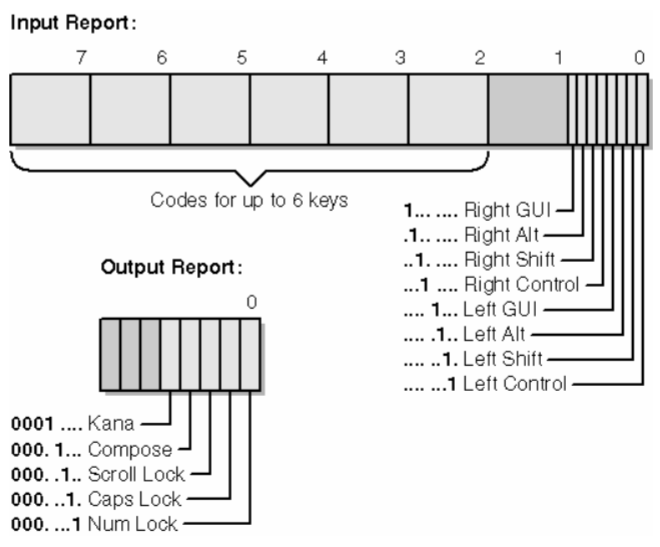
\includegraphics[width=\textwidth]{images/mk02.png}
    \caption{Struktura raportu~\cite{oney}}
    \label{fig:report}
\end{figure}
Implementacja symulowania działania klawiatury będzie polegała na implementacji generowania prawidłowych raportów wejściowych.
Obsługę raportów wejściowe można zignorować. Nie jest ona wymagana do poprawnego działania systemu, ponieważ zapalanie odpowiednich indykatorów nie jest częścią wymagań funkcjonalnych.
Wartości, jakie należy nadać poszczególnym bajtom, aby wskazać wciśnięcie danego klawisza można odczytać z przytoczonego już \textit{HID Usage Tables}. 
Warto mieć na uwadze, że nie ma żadnego powiązania z kodami ASCII. Przykładowo wartość zarówno dla znaków 'a' oraz 'A' to 04h (rozróżnia je odpowiedni modyfikator przesyłany w pierwszym bajcie), podczas gdy w ASCII to odpowiednio 61h i 41h. Obsługa kodu klawisza wysyłane przez urządzenia HID może się różnić w zależności od systemu operacyjnego, np. tylko system MacOS obsługuje kody klawiszy od F13 do F15~\cite{hut}.

\subsection[Konfiguracja]{Konfiguracja}
Do skonfigurowania urządzenia wykonującego jako kartę sieciową wykorzystujemy wsparcie platformy dla \textit{usb gadget modes}. Jest to możliwe dzięki złączu Universal Serial Bus (USB) znajdującemu się na płytce Raspberry Pi Zero mogącemu pracować w trybie \textit{On-The-Go} (OTG). Oznacza to, że urządzenie może zmieniać swoją rolę pomiędzy \textit{host} i \textit{slave}. W przypadku działania urządzenia jako karta sieciowa potrzebny jest tryb \textit{slave}, który nazywany jest też \textit{device}. Konieczne są również odpowiednie moduły jądra systemu Linux dostarczone przez system \textit{Raspbian}, które za pomocą odpowiedniej konfiguracji zostają załadowane do systemu. W zależności, który z nich zostanie wybrany realizowana będzie inna funkcjonalność. W tym przypadku jest to g\_ether - ethernet gadget driver oraz dwc2 - sterownik zajmujący się obsługą funkcjonalności USB OTG.
Po załadowaniu wyżej wymienionych modułów możliwe jest korzystanie z interfejsu \textit{usb0}, jednak trzeba go skonfigurować. Nadajemy statyczny adres IP aby możliwe było późniejsze jednoznaczne odwoływanie się do niego (patrz listing~\ref{lst:ifconfig}).
\begin{lstlisting}[language=bash,caption={Konfiguracja interfejsu \textit{usb0}},label={lst:ifconfig}]
    ifconfig usb0 192.168.100.1 netmask 255.255.255.0 up
\end{lstlisting}
W celu automatycznej konfiguracji hosta z pomocą DHCP zastosowano serwer \textit{Dnsmasq}. Pozwala to na automatyczne przypisanie adresu IP do interfejsu,
do którego podpięty został kabel USB w testowanym komputerze. Do poprawnego działania serwera konieczne jest edytowanie pliku konfiguracyjnego \textit{/etc/dnsmasq.conf}.
Należy ustawić interfejs oraz adres IP, na którym nasłuchiwać mają usługi DHCP i DNS oraz pulę adresów IP (patrz listing~\ref{lst:dhcp}).\newpage
\begin{lstlisting}[language=bash,caption={Konfiguracja serwera DHCP},label={lst:dhcp}]
    interface=usb0
    listen-address=192.168.100.1
    dhcp-range=192.168.100.50,192.168.100.150,12h 
\end{lstlisting}
Następnie należy włączyć \textit{IP forwarding}, aby możliwe było przekazywanie pakietów pomiędzy interfejsami \textit{usb0} oraz \textit{wlan0}.
Konfigurujemy je za pomocą polecenia iptables, w którym określamy reguły przepływu pakietów (patrz listing~\ref{lst:iptables}). 
\begin{lstlisting}[language=bash,caption={Ustawianie reguł przepływu pakietów},label={lst:iptables}]
    iptables -t nat -A POSTROUTING -o wlan0 -j MASQUERADE
    iptables -A FORWARD -i wlan0 -o usb0 -m state --state RELATED,ESTABLISHED -j ACCEPT
    iptables -A FORWARD -i usb0 -o wlan0 -j ACCEPT 
\end{lstlisting}
\begin{enumerate}
    \item Wszystkie pakiety opuszczające urządzenie przez interfejs \textit{wlan0}, są poddawane operacji maskarady, która poprawia bezpieczeństwo ukrywając wewnętrzne adresy IP w danej sieci.
    \item Akceptacja przekazywania pakietów z interfejsu \textit{wlan0} do interfejsu \textit{usb0}
    \item Akceptacja przekazywania pakietów z interfejsu \textit{usb0} do interfejsu \textit{wlan0}
\end{enumerate}

\subsection[Wykrywalnosc (Jakub Wyka)]{Wykrywalność złośliwego urządzenia USB w konfiguracji karty sieciowej}
\label{subsec:wykrywalnoscJW}

W systemie \textit{Windows} podczas konfiguracji urządzenia pojawia się okienko systemowe opisane wcześniej w
 sekcji~\ref{subsec:wykrywalnoscMK}. Poza nim, po udanej konfiguracji urządzenia wykonującego
 jako karta sieciowa, wyświetla się okno informujące o połączeniu z nową siecią, mimo że
 użytkownik systemu nie łączył się z nią świadomie.
  Jest to prawidłowa reakcja systemu, która może spowodować, że użytkownik, posiadający 
  podstawową wiedzę na temat działania komputera, wykryje złośliwe urządzenie. 


  \begin{figure}[H]
    \centering
    
\includegraphics[width=0.5\textwidth]{newcon}
    \caption{Interfejs wyświetlany po udanym połączeniu z nową siecią}
    \label{fig:newcon}
\end{figure}
\subsection[Scenariusz - Pharming (Jakub Wyka)]{Scenariusz - Pharming}

\subsubsection[Założenia początkowe]{Założenia początkowe}

    
Urządzenie wykonujące powinno być podłączone do internetu za pomocą sieci wi-fi oraz połączone
z testowanym komputerem za pomocą przewodu usb - micro usb. Ważne jest również aby było podłączone
do serwera, który zarządza wykonywaniem testów.
Ważne jest również aby osoba wykonująca test - Pentester, była zalogowana do serwera.

\subsubsection[Aktorzy]{Aktorzy}
\begin{itemize}
    \item 	Pentester
    \item 	Serwer sterujący
    \item 	Testowany system
    \item   Urządzenie wykonujące
\end{itemize}
\subsubsection[Opis testu]{Opis testu}
Zatruwanie DNS to metoda ataku polegająca zmianie lokalnego rekordu DNS, który
fałszywie przypisuje nazwę domeny do adresu IP.  
Zadaniem tego ataku jest przekierowanie użytkownika na inną stronę niż ta,
 którą faktycznie chciał otworzyć. Często witryna podszywająca się wygląda 
 tak samo, przez co użytkownik nie jest świadomy ataku. Podszywanie to jest 
 nazywane phishingiem. W ten sposób użytkownik logując się do serwisu dostarcza 
 wrażliwe dane osobom przeprowadzającym atak. Połączenie DNS spoofingu z 
 zaawansowanym phishingiem nazywane jest pharmingiem.

 \subsubsection[Przebieg testu]{Przebieg testu}
Serwer sterujący służy do wydawania poleceń przez pentestera. 
Wybiera on, za pomocą którego z dostępnych urządzeń testujących 
ma zostać przeprowadzony test. Następnie wybiera rodzaj testu. W tym 
przypadku będzie to pharming. Serwer udostępni możliwość określenia
 konkretnych parametrów testu. Dla tego typu testy będzie to rekord DNS,
  który określi pod jaką domenę chcemy się podszyć oraz ip strony podszywającej. 
  Serwer przesyła te dane do urządzenia wykonującego, które na tej podstawie uruchamia 
  skrypt, który jest odpowiedzialny za przeprowadzenie testu. Do serwera odsyłany
jest raport z wynikiem testu. 
\begin{figure}[H]
    \centering
    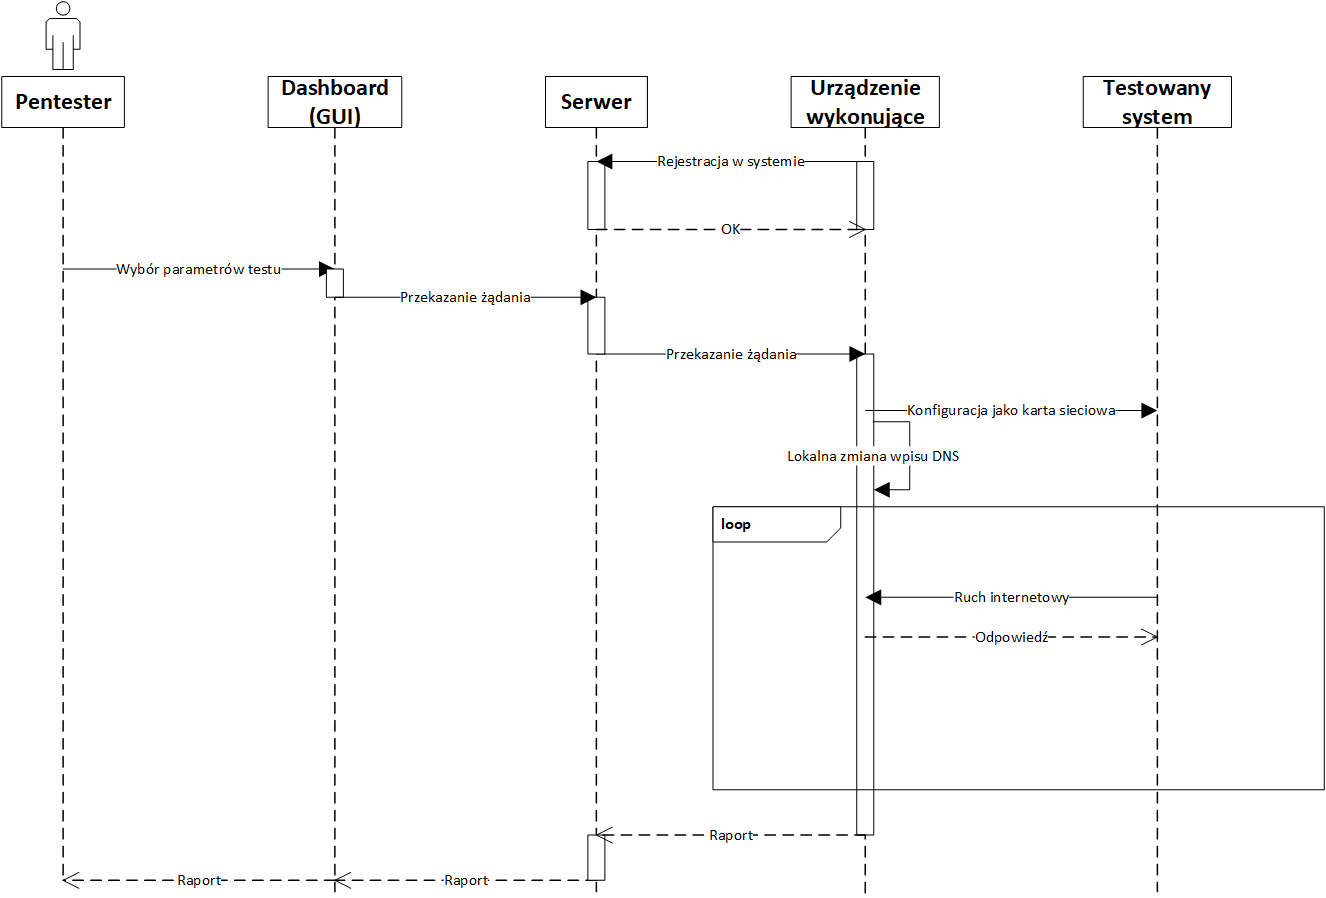
\includegraphics[width=\textwidth]{interJW}
    \caption{Diagram interakcji dla scenariusza testowego "Pharming"}
    \label{fig:pharming1}    
\end{figure}
\begin{figure}[H]
    \centering
    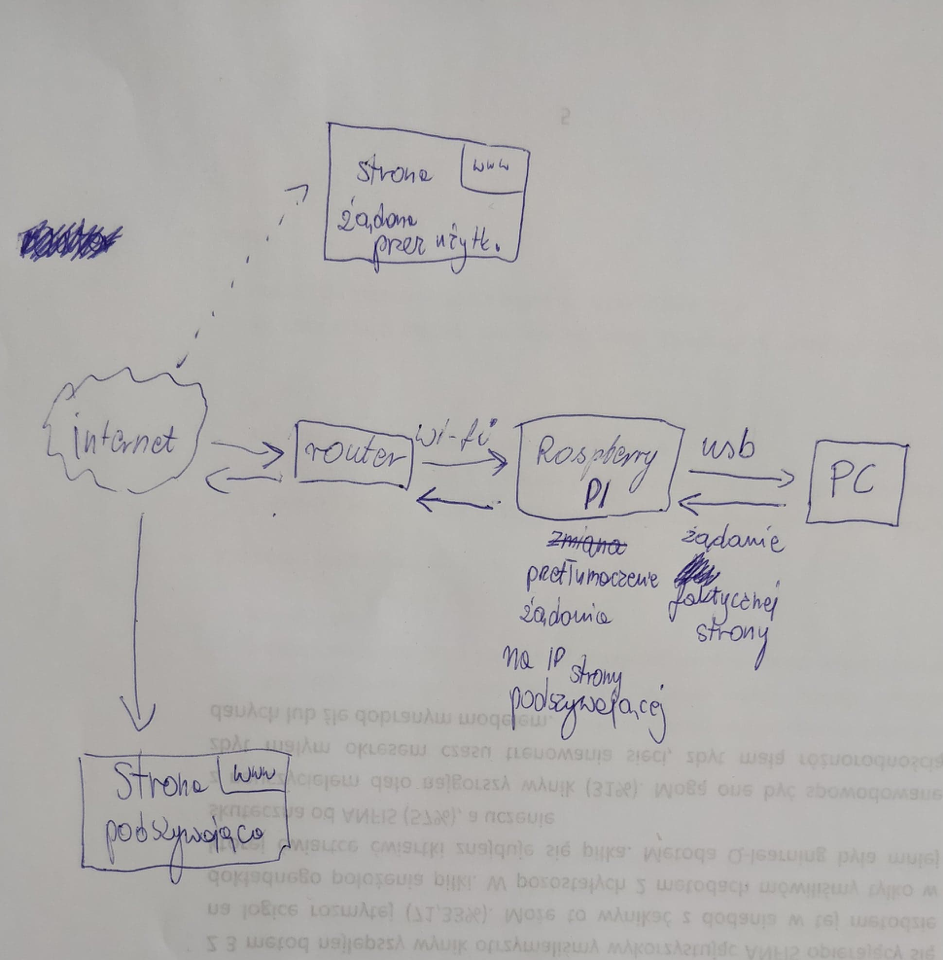
\includegraphics[width=\textwidth]{jw03}
    \caption{Pharming2}
    \label{fig:pharming2}    
\end{figure}

\subsubsection[Mozliwosc wykrycia]{Możliwość wykrycia }

Phishing jest metodą oszustwa opartą na inżynieri społecznej.
Ten scenariusz testowy ma więc na celu przetestowanie zachowania człowieka, który jest użytkownikiem systemu.
Wynika to z faktu, że jego głównym celem jest przekierowanie go na podszywającą się witrynę i
 wydobycie od niego wrażliwych danych. Należy więc zauważyć, że podmiana rekordu dns jest jedynie środkiem
 do udanego przeprowadzenia symulacji ataku phishingowego.
 Alternatywnym sposobem mogłoby być rozesłanie wiadomości drogą elektroniczą ze złośliwym hiperłączem, jednak
 atutem rozwiązania korzystającego z urządzenia USB jest możliwość przetestowania świadomości użytkowników
 na temat niebezpieczeństw jakie niosą nieznane urządzenia podłączane do systemu.

Możliwość wykrycia złośliwego urządzenia w konfiguracji karty sieciowej została opisana w sekcji ~\ref{subsec:wykrywalnoscJW},
więc w tym rozdziale opisana zostanie taka możliwość dla phishingu.
Kluczowe w dbaniu o autentyczność witryny są certyfikaty SSL. Istotny jest również ich rodzaj, gdyż wyróżniamy\cite[]{ssltypes}:
\begin{itemize}
    \item Domain Validation SSL certificates (DV) 
    \subitem Jest to najszybszy i najprostszy sposób uzyskania certyfikatu SSL. 
    \item Organization Validation (OV)
    \subitem Aby uzyskać ten certyfikat należy przejść głębszą weryfikację.
    \item Extended Validation SSL certificates (EV)
    \subitem Certyfikat zapewnia wyższy poziom zaufania i bezpieczeństwa, dzięki długiemu procesowi
    weryfikacji. Trwa ona nawet kilka tygodni, przez co jest kosztowna.
    Jednak najważniejsze jest to, że został zaprojektowany tak aby zapewniać ochronę przed
    atakami typu phishing.      
\end{itemize}

Podsumowując, użytkownicy powinni zwracać uwagę na obecność Extended Validation SSL certificate. Okazuje się,
że wbrew popularnej opinii, samo posiadanie certyfikatu ssl może nie być  wystarczające aby jednoznacznie stwierdzić bezpieczeństwo witryny.
\begin{figure}[H]
        \centering
        
\includegraphics[width=\textwidth]{ev}
        \caption{Przykład wizualizacji posiadania certyfikatu EV przez daną witrynę, zaczerpnięty z \cite[]{sslev}}
        \label{fig:ev}
    \end{figure}
\subsection[Scenariusz - man in the middle (Michał Krakowiak)]{Scenariusz - man in the middle}
\label{sce:mitm}
Jednym z powszechniejszych zagrożeń sieciowych jest tzw. \textit{man in the middle}, czyli w dosłownym tłumaczeniu \textit{człowiek w środku}.
W takim scenariuszu napastnik pośredniczy w połączeniu internetowym danego systemu komputerowego.
W związku z tym wszystkie wysyłane i odbierane mogą być przechwycone oraz potencjalnie zmodyfikowane.
Tworzy to niebezpieczeństwo m.in. kradzieży ciasteczek, wstrzyknięcia javascript do zapytania oraz bardziej zaawansowanych ataków na połączenia szyfrowane jak SSLsplit.
\subsubsection[Aktorzy]{Aktorzy}
\begin{itemize}
    \item Pentester – osoba przeprowadzająca test bezpieczeństwa systemu komputerowego za pomocą dedykowanego systemu
    \item Urządzenie wykonujące – niewielkie urządzenie oparte o platformę Raspberry Pi Zero W, podłączone za pomocą portu USB do testowanego systemu
    \item Środowisko testowe – centralny punkt infrastruktury, rejestruje aktywne urządzenia wykonujące, przyjmuje polecenia od testera, przekazuje je do wskazanych urządzeń wykonującyc.
    \item Testowany system – system komputerowy pracujący pod kontrolą systemu operacyjnego \textit{Windows 10}, użytkownik nie posiada uprawnień administratora
\end{itemize}
\subsubsection[Przebieg]{Przebieg}
Test bezpieczeństwa korzystający realizowanego systemu rozpoczyna się od dostarczenia i instalacji skonfigurowanego urządzenia wykonującego.
Uruchomiony system komputerowy dostarczy zasilanie urządzeniu po przez port USB.
Podczas swojego startu urządzenie wykonujące uruchamia skrypt odpowiedzialny za obsługę komunikacji z środowiskiem testowym oraz obsługę połączenia USB.
Resztę działań tester przeprowadza zdalnie. Z poziomu przeglądarki ma dostęp do aplikacji która pozwala wskazać jedno lub więcej urządzeń zarejestrowanych w systemie.
Następnie przygotowuje odpowiedni dla testu payload, w którym wskazuje takie elementy jak:
\begin{itemize}
    \item tryb działania: tylko podsłuch czy wstrzykiwanie kodu
    \item ilość datagramów IP, które mają zostać podsłuchane
    \item kod html lub javascript, który zostanie dołączony do określonej liczby odpowiedzi HTTP
\end{itemize}

Po poprawnym przyjęciu żądanej operacji pentester wykorzystując środowisko testowe wysyła wiadomość z ładunkiem do wskazanych urządzeń.
Identyfikują one polecenie i rozpoczyna wykonywanie skryptów inicjujących wymagane funkcjonalności. Uwzględnia to ewentualną zmianę z innych zrealizowanych trybów pracy.
Urządzenie wykonujące rejestruje swoją obecność w testowanym systemie komputerowym jako zewnętrzna karta sieciowa.
Następnie rozsyłane są odpowiednio spreparowane ustawienia DHCP dla nowo przyłączonego interfejsu sieciowego w testowanym systemie.
Zapewniają, że ruch sieciowy będzie kierowany na spreparowaną kartę sieciową, a następnie obsługiwany w żądany sposób.
Sposób działania urządzenia powinien być możliwie transparentny.
\begin{figure}[H]
    \centering
    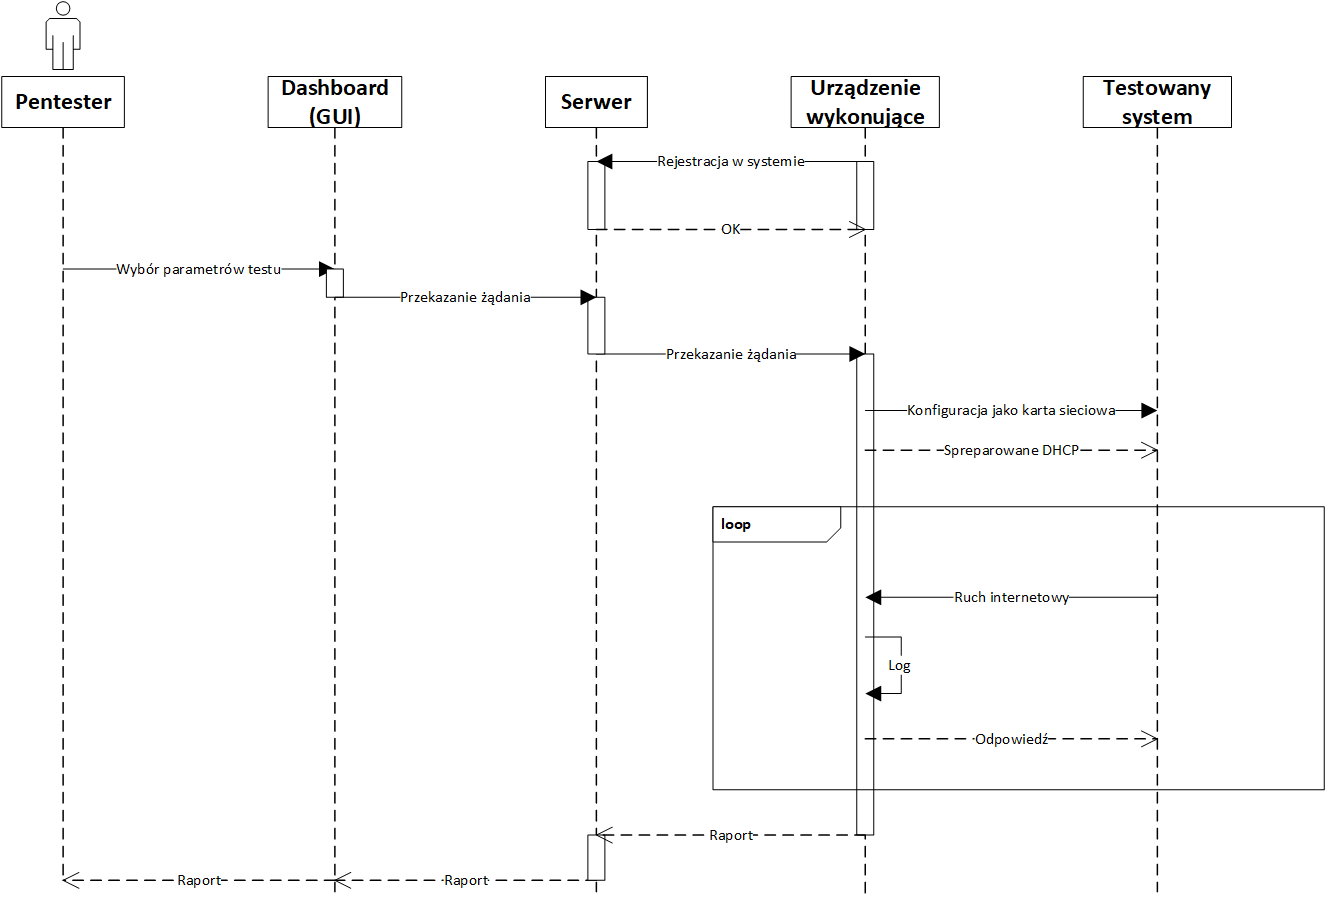
\includegraphics[width=\textwidth]{interakcjaMK}
    \caption{Diagram interakcji dla scenariusza testowego \textit{MITM}}
    \label{fig:mitm}    
\end{figure} \newpage
\section[Rezultaty]{Rezultaty}
\label{chapter:results}
Utworzony system ma na celu badanie bezpieczeństwa, natomiast rezultatem jest możliwość przeprowadzenia testów. Testy pokazują występowanie podatności. 
Do oceny ryzyka wskazanej podatność zostanie wykorzystany model DREAD (ang. Damage, Reproducibility, Exploitability, Affected users, Discoverability). System oceniania polega na przydzieleniu każdej z pięciu kategorii wartość od 1 do 10. Im wyższa ocena, tym ryzyko jest większe.  
\begin{itemize}
    \item Szkody (ang. Damage) oznacza, jak duże mogą być konsekwencje wykorzystania podatności
    \item Odtwarzalność (ang. Reproducibility) oznacza, jak łatwo można wykorzystać podatność
    \item Możliwość wykorzystania (ang. Exploitability), mówi o tym, ile czasu jest potrzebne do uruchomienia potencjalnego ataku
    \item Dotknięci użytkownicy (ang. Affected users), ta kategoria ocenia podatność pod względem liczby poszkodowanych osób
    \item Wykrywalność (ang. Discoverability), ocena pod względem wykrywalności zagrożenia, to znaczy jak łatwo użytkownik zorientuje się, że jest (lub był) atakowany
\end{itemize}

\subsection[Podatności na podszywanie się pod HID]{Podatności na podszywanie się pod HID}
\subsubsection[Wykazanie podatności]{Wykazanie podatności}
Scenariusz~\ref{sce:klawiatura} opisuje test polegający na zdalnym wprowadzeniu dowolnej sekwencji klawiszy w systemie komputerowym. Zostały w nim zawarte niezbędne informacje do przeprowadzenia testu podatności. Scenariusz opisuje urządzenia oraz założenia początkowe wymagane do poprawnego wykonania testu. Najważniejszym urządzeniem jest platforma wykonującą (tzn. rpi identyfikujący się jako klawiatura), którą pentester podłącza do komputera z systemem \textit{Windows}. Po podłączeniu pentester przygotowuje payload. Przykład na listinigu~\ref{lst:hid}.
\begin{lstlisting}[language={},label={lst:hid},caption={Przykładowy payload}]
{
    'deviceType': 'KEYBOARD',
    'name': 'test',
    'idVendor': '0x1d6b',
    'idProduct': '0x0104',
    'serial': 'fedcba9876543210',
    'manufacturer': 'BSC',
    'product': 'BSC',
    'payloads':[{'delay':0.5,'key':'r','leftGUI':'True'},
                {'delay':0.5,'text':'cmd.exe\\n'}]
}
\end{lstlisting}
Pierwsze elementy odpowiadają za konfigurację urządzenia, z kolei ostatni \textit{payloads} zawiera listę komend (tzn. sekwencje klawiszy które mają zostać wysłane). W przedstawionym ładunku pierwsza komenda ma zadanie uruchomić okno umożliwiające włączenie dowolnego programu. Skrót odpowiadający za uruchomienie tego okna w systemie \textit{Windows} to \textit{win + r}, gdzie klawiszowi \textit{win} odpowiada \textit{leftGUI}. W kolejnym argumencie został podany tekst \textit{cmd.exe}, który zostanie podany na wejście. Wynikiem obsłużenia przedstawionego ładunku, będzie otworzenie konsoli, następnie można podać kolejne argumenty, które wyślą dowolną inną kombinację klawiszy. Pentester, może ustawić opóźnienie, wykonania komendy.
Pentester może w każdym momencie wysłać nowy ładunek na aktywne urządzenie wykonujące za pośrednictwem interfejsu użytkownika. Przykładowy payload z listingu~\ref{lst:hid}, pozwala na uruchomienie konsoli. Dalej można zlecić kolejne instrukcje, np. skrypt powłoki, uzyskując podatność typu RCE. 
\subsubsection[Ocena Ryzyka]{Ocena Ryzyka}
\begin{itemize}
    \item Szkody - duże, szkody spowodowane przez zdalne wykonywanie kodu mogą być bardzo duże i nie są zależne od uprawnień zalogowanego użytkownika. Pomimo braku pełnych praw administratora pentester może eskalować uprawnienia, wykorzystując inne luki. Podatność RCE daje narzędzia do przejmowania danych oraz wykonywania skryptów.
    \item Odtwarzalność - średnia, nie jest łatwa ze względu na to, że pentester musi mieć kontakt fizyczny z testowanym komputerem lub nieświadomy użytkownik podłączy urządzenie. Przez fakt, że następuje postęp miniaturyzacja elektroniki oraz wiele osób jest nieświadomych zagrożeń wynikających z wpinania niesprawdzonego sprzętu ocena odtwarzalności klasyfikuje się na średnim poziomie. Szerszy opis znajduje się w rozdziale~\ref{bez:int}. %Natomiast w momencie, gdy platforma wykonujące jest już podłączona odtwarzalność jest już dużo prostsza ponieważ pentester może w dowolnej chwili wykonać test.
    \item Możliwość wykorzystania - średnia, uruchomienie testu zajmuje kilkadziesiąt sekund z czego większość jest poświęcona na konfigurację wstępną platformy wykonującej. %Szerzej zostało opisane w rozdziale 
    \item Dotknięci użytkownicy - średnia, potencjalnym celem może być osoba aktualnie zalogowana lub inne osoby korzystający  z komputera, w przypadku gdy zalogowany użytkownik ma uprawnienia administratora lub pentester wykorzysta inne luki do zdobycia tych uprawnień.
    \item Wykrywalność - mała, poziom jest dosyć niski, gdyż opóźnienie przy wysyłaniu kolejnych sekwencji znaków jest minimalne i nieświadomy użytkownik może się nie zorientować, że właśnie został wykonany kod. Po podłączeniu i uruchomieniu urządzenia system \textit{Windows} informuje o nierozpoznanym urządzeniu, lecz większość nieświadomych użytkowników może zignorować komunikat.
\end{itemize}
\subsection[Podatność na zatruwanie DNS (Jakub Wyka)]{Podatność na zatruwanie DNS}
\subsubsection[Wykazanie podatności]{Wykazanie podatności}
W rozdziale~\ref{chapter:usbethernet} omawiana była realizacja symulowania działania karty sieciowej.
W ramach tej funkcjonalności powstał scenariusz (rozdział~\ref{sce:phar}) 
zakładający zmianę rekordu DNS. W celu przeprowadzenia testu należy przesłać odpowiednio przygotowaną 
wiadomość do urządzenia wykonującego. 

\begin{lstlisting}[language={},label={lst:ph},caption={Przykładowa wiadomość}]
    {
        {
            'deviceType': 'ETHER',
            'name': 'test',
            'idVendor': '0x1d6b',
            'idProduct': '0x0104',
            'serial': 'fedcba9876543210',
            'manufacturer': 'BSC',
            'product': 'BSC',
            'payloads':
            [
                {
                    'scenario': 'SPOOFING',
                    'params': 
                    [
                        {
                            'ipAddress': '192.168.1.1',
                            'hostname': 'wp.pl',
                            'duration':'240'
                        }
                    ]
                }
            ]
        }
    }
\end{lstlisting}
Jak już wspomniano w rozdziale ~\ref{chapter:mitmMK} przykładowa konfiguracja z listingu~\ref{lst:ph} 
zawiera podstawowe parametry konfiguracyjne dla tworzonego gadżetu USB. Należy również podać 
nazwę realizowanego scenariusza. W tym przypadku jest to \textit{SPOOFING}.
Za pomocą pola \textit{params} przekazywane są parametry specyficzne 
dla wybranego wcześniej scenariusza. 
Jest to \textit{ipAddress}  który określa adres IP w dodawanym rekordzie DNS, a nazwę 
hosta definiuje pole \textit{hostname}. \textit{Duration} jest parametrem określającym czas 
trwania testu. Powyższe parametry wystarczają aby dodać lokalny wpis DNS na urządzeniu wykonującym 
i przekierować użytkownika systemu do złośliwej witryny. Jeśli podany adres IP odpowiada adresowi 
przypisanemu do interfejsu wlan0 urządzenia wykonującego, użytkownik zostaje przekierowany do dokumentu 
hostowanego przez serwer http na urządzeniu wykonującym. Za pomocą skryptu php wpisane przez niego 
wrażliwe dane zostają zapisane na dysku, a następnie zostają odesłane w raporcie testu.

\subsubsection[Ocena Ryzyka]{Ocena Ryzyka}
\begin{itemize}
    \item Szkody - duże, przekierowanie użytkownika na stronę podszywającą się bez jego 
    wiedzy może przynieść poważne konswekwencje. W szczególności jest to kradzież wrażliwych 
    danych, które mogą zostać wykorzystane m.in. do kradzieży konta na portalu lub dostęp do 
    konta bankowego. Oznaczać to może stratę faktycznych dóbr materialnych przez ofiarę.
    \item Odtwarzalność - średnia, opisana w rozdziale ~\ref{chapter:ormitm}.
    \item Możliwość wykorzystania - średnia, opisana w rozdziale ~\ref{chapter:ormitm}.
    \item Ilość dotkniętych użytkowników - mała, zmiana rekordu DNS dotyczy tylko użytkownika, 
    do którego stacji roboczej podłączone jest urządzenie wykonujące.
    \item Wykrywalność - średnia, opisana w rozdziałach ~\ref{subsec:wykrywalnoscJW} i ~\ref{subsec:wykrpharming}. 
    Użytkownik jest w stanie wykryć symulację ataku, jednak wymaga to od niego podstawowej wiedzy na temat 
    certyfikatów. Ważne jest też zwracanie uwagi na komunikaty systemowe.
\end{itemize}

\subsection[Podatność na przechwycenie ruchu sieciowego (Michał Krakowiak)]{Podatność na przechwycenie ruchu sieciowego}
\subsubsection[Wykazanie podatności]{Wykazanie podatności}
\label{chapter:mitmMK}
W rozdziale~\ref{chapter:usbethernet} omawiana była realizacja symulowania działania karty sieciowej.
W ramach tej funkcjonalności powstał scenariusz (rozdział~\ref{sce:mitm}) zakładający przechwycenie ruchu sieciowego.
W celu przeprowadzenia testu system należy odpowiednio uzbroić, przekazując wymaganą konfigurację.
\begin{lstlisting}[language={},label={lst:mitm},caption={Przykładowa konfiguracja}]
{
    'deviceType': 'ETHER',
    'name': 'test',
    'idVendor': '0x1d6b',
    'idProduct': '0x0104',
    'serial': 'fedcba9876543210',
    'manufacturer': 'BSC',
    'product': 'BSC',
    'nfqueue': True,
    'payloads': [
        {
            'scenario': 'INJECT',
            'code': '<script>alert(\"Hello World\");</script>',
            'count': 3
        }
    ]
}
\end{lstlisting}
Przykładowa konfiguracja z listingu~\ref{lst:mitm} zawiera podstawowe parametry konfiguracyjne dla tworzonego gadżetu USB.
Pojawia się pole \textit{nfqueue} (skrócona nazwa pochodząca od \textit{netfilter queue}), które jest odpowiedzialne za poinformowanie systemu o konieczności przekierowania ruchu sieciowego do dedykowanej kolejki.
\textit{Netfilter queue} pozwala na filtrowanie i modyfikowanie przekierowanych do niej danych z poziomu przestrzeni adresowej użytkownika.
W związku z implementacją więcej niż jednego scenariusza z wykorzystaniem symulowanej karty sieciowej wymagane jest wskazanie oczekiwanej funkcjonalności (pole \textit{scenario}).
Test wykorzystuje fakt, że po przyłączeniu nowego interfejsu system \textit{Windows~10} decydował o kierowaniu do niego wszystkie dane.
System nie zweryfikował autentyczności nowego interfejsu.
Takie zachowanie umożliwiło wykorzystanie pośredniczenia w połączeniu.
Dedykowany system był wstanie przechwycić każdą przesłaną informację.
Na potrzeby analizy krytyczności zagrożenia wprowadzono obsługę modyfikacji nagłówków HTTP:
\begin{itemize}
    \item podmianę wersji protokołu na 1.0
    \item ustawienie preferowanej zawartości danych jako zwykły tekst
    \item aktualizacja rozmiaru danych HTTP.
\end{itemize}
Pozwoliło to wstrzyknąć kod i wykonać przesłany w ładunku.
Daje to możliwość dalszej eskalacji i wykorzystania innych podatności.
Warunkiem pomyślnej exploitacji jest obecność niezaszyfrowanego ruchu, od którego już się odchodzi.
\subsubsection[Ocena ryzyka]{Ocena ryzyka}
\label{chapter:ormitm}
Na podstawie przeprowadzonego testu stwierdzono średnie ryzyko zagrożenia. Szczegółowa ocena:
\begin{itemize}
    \item Szkody - duże, obecność zdalnie sterowanego urządzenia w połączeniu internetowym daje takie możliwości przechwytywanie plików cookie lub wstrzyknięcie kodu javascript
    \item Odtwarzalność - średnia, odtworzenie scenariusza wymaga dostępu do fizycznego interfejsu komputera, jednak należy uwzględniać, że koszt miniaturowej elektroniki maleje; złośliwe urządzenia mogą być dystrybuowane z wykorzystaniem metod socjotechnicznych (np. w postaci darmowych gadżetów reklamowych)  
    \item Możliwość wykorzystania - średnia, skuteczne wykorzystanie wymaga nie tylko odpowiedniego oprogramowania, ale też dystrybucji fizycznego urządzenia
    \item Ilość dotkniętych użytkowników - mała, skuteczne wykorzystanie przejęcia ruchu sieciowego zagraża przede wszystkim użytkownikom danego systemu komputerowego
    \item Wykrywalność - średnia, szerzej opisana w rozdziałach~\ref{subsec:wykrywalnoscMK} i~\ref{subsec:wykrywalnoscJW}, użytkownik ma szansę wykryć zagrożenie, jednak zignorowanie komunikatu w przypadku nieświadomych użytkowników może skutkować utrudnieniami w późniejszym wykryciu.
\end{itemize} \newpage
\section[Podsumowanie (Michał Krakowiak, Kacper Połom, Jakub Wyka)]{Podsumowanie}
\label{chapter:summary}
Temat pracy inżynierskiej \textit{System dedykowany wspomagający testowanie bezpieczeństwa systemu komputerowego}
jasno określa zawartość tego dokumentu. Tekst skupia się na bezpieczeństwie systemu 
komputerowego uwzględniając wszystkie jego składowe. 
\begin{itemize}
    \item warstwę fizyczną
    \item oprogramowanie
    \item użytkownika
\end{itemize}
Spośród wielu możliwych testów bezpieczeństwa wybrano takie, które 
dotyczą wszystkich przedstawionych wyżej aspektów. W tym celu zdecydowano, że 
zastosowany zostanie sprzętowy komponent w postaci urządzenia wykonującego skrypty testowe. 
Dzięki temu każdy scenariusz testowy sprawdza świadomość użytkownika dotyczącą 
niezaufanych urządzeń podłączanych do stacji roboczej. Następnie wybrany został obszar 
testów bezpieczeństwa wzorowanych na prawdziwych atakach wymierzonych w systemy komputerowe. 
Zdecydowano aby oprzeć ten projekt na testach bezpieczeństwa związanych z 
symulowaniem działania klawiatury oraz kradzieży
wrażliwych danych użytkownika korzystającego z sieci internet.


Realizacja projektu wspomagającego ofensywne testy bezpieczeństwa jest wymagająca przez względy prawne.
Wciąż oczekuje się nowych przejrzystszych regulacji dotyczących testów penetracyjnych i programów bug bounty.
Na każdym etapie implementacji należało podkreślać cel pracy, jakim jest pomoc w zabezpieczaniu zlokalizowanych słabych punktów systemu komputerowego.
Ponadto otrzymane rezultaty uświadamiają jakim zagrożeniem stała się możliwość oprogramowywania urządzeń USB.
Brak autoryzacji akcesoriów pozwala wprawdzie na bezproblemowe i niemal natychmiastowe ich działanie, ale nadużycie zaufania wydaje się dosyć dużym zagrożeniem.

-- wnioski z 4 rozdziału KP

Przedstawiony system spełnia założenia projektowe i z powodzeniem może być wykorzystywany 
do realizacji swojego głównego celu, jakim jest testowanie bezpieczeństwa systemów 
komputerowych. Jego implementacja przebiegła pomyślnie. 

Dalszy rozwój systemu mógłby się opierać na dodaniu nowych scenariuszy testowych 
do już istniejących konfiguracji karty sieciowej oraz klawiatury. 
W związku z tym system umożliwia łatwą rozbudowę o nowe skrypty testujące bezpieczeństwo.
Jeszcze ciekawsze wydaje się dodanie nowej konfiguracji urządzenia wykonującego takiego jak: kamerka internetowa, drukarka lub 
pamięć masowa, wykorzystując sterowniki systemu Linux.
 \newpage

\renewcommand{\baselinestretch}{1.0}\normalsize	% żeby w wykazach była pojedyncza interlinia

\clearpage
\addcontentsline{toc}{section}{Wykaz literatury}
\nocite{*}
\printbibliography
\newpage

\renewcommand{\listfigurename}{Wykaz rysunków}
\addcontentsline{toc}{section}{\listfigurename}
\listoffigures
\newpage

\renewcommand{\listtablename}{Wykaz tabel}
\addcontentsline{toc}{section}{\listtablename}
\listoftables

\renewcommand{\baselinestretch}{1.5}\normalsize	% powrót do interlinii 1.5 na wypadek dodatków

% nie dodawaj obrazków i tabel z dodatków do list powyżej
\let\svaddcontentsline\addcontentsline
\renewcommand\addcontentsline[3]{%
  \ifthenelse{\equal{#1}{lof}}{}%
  {\ifthenelse{\equal{#1}{lot}}{}{\svaddcontentsline{#1}{#2}{#3}}}}

\newpage

\begin{appendices}
\addtocontents{toc}{\protect\setcounter{tocdepth}{1}}

\renewcommand{\appendixname}{Dodatek}
%\input{chapters/appendix} \newpage
\end{appendices}

\end{document}	% musi być na samiutkim końcu
